\section[Major Contribution 1]{Major Contribution 1: Application-Specific Fault Tolerance}

\begin{frame}
  \frametitle{ULFM: User-Level Failure Mitigation}

  \centering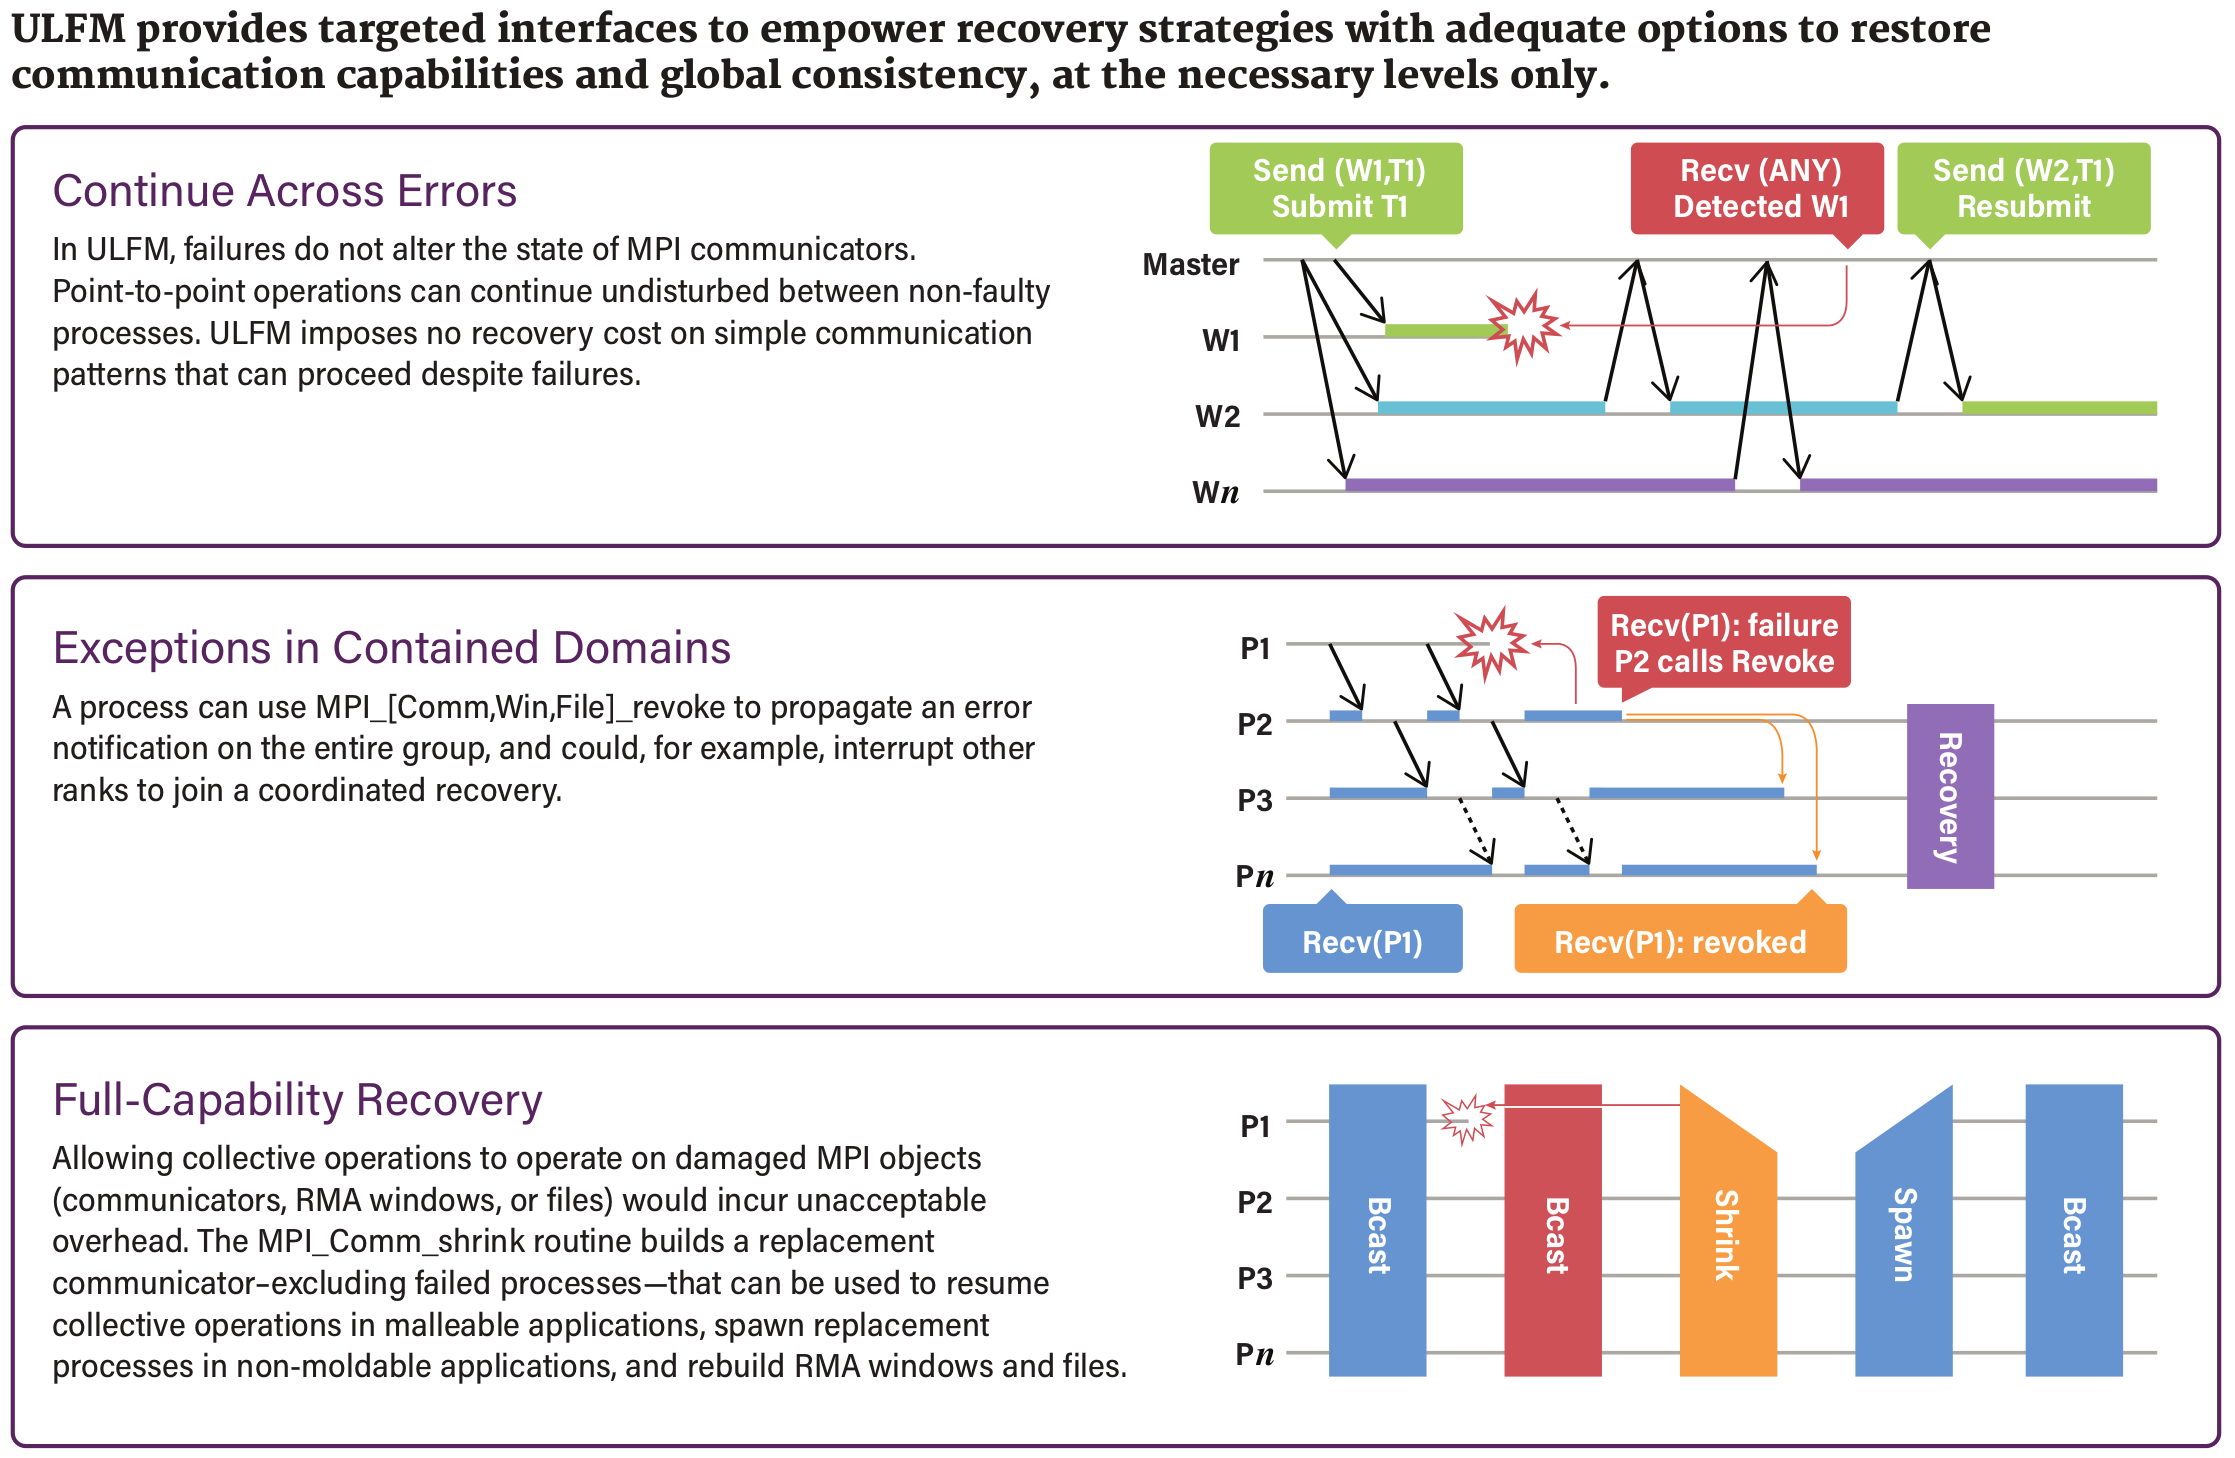
\includegraphics[height=.85\textheight]{ulfm.png}

\end{frame}


\newcommand{\processes}{\ensuremath{{\mathcal P}}}
\newcommand{\status}[2]{\ensuremath{S_{#1}^{#2}}}
\newcommand{\emitter}{\ensuremath{\texttt{emitter}}\xspace}
\newcommand{\observer}{\ensuremath{\texttt{observer}}\xspace}
\newcommand{\alive}{\ensuremath{\texttt{alive}}\xspace}
\newcommand{\dead}{\ensuremath{\texttt{dead}}}
\newcommand{\heartbeat}{\ensuremath{\textsc{heartbeat}}\xspace}
\newcommand{\timeoutping}{\ensuremath{\textsc{HB-Timeout}}\xspace}
\newcommand{\timeoutsuspect}{\ensuremath{\textsc{Susp-Timeout}}\xspace}
\newcommand{\timeout}[1]{\ensuremath{\textsc{Timeout}_{#1}}\xspace}
\newcommand{\newobserver}{\ensuremath{\textsc{NewObserver}}\xspace}
\newcommand{\findpred}{\ensuremath{\textit{FindEmitter}}\xspace}
\newcommand{\neighbors}{\ensuremath{\textit{Neighbors}}\xspace}
\newcommand{\broadcastmsg}{\ensuremath{\textsc{BcastMsg}}\xspace}
\newcommand{\pinginterval}{\ensuremath{\eta}\xspace}
\newcommand{\msgtime}{\ensuremath{\tau}\xspace}
\newcommand{\suspectinterval}{\ensuremath{\delta}\xspace}
\newcommand{\emittors}[1]{\ensuremath{M(#1)}}
\newcommand{\ringemittor}[1]{\ensuremath{M_R(#1)}}
\newcommand{\additionalemittors}[1]{\ensuremath{M_A(#1)}}
\newcommand{\receivers}[1]{\ensuremath{O(#1)}}
\newcommand{\ringreceiver}[1]{\ensuremath{O_R(#1)}}
\newcommand{\additionalreceivers}[1]{\ensuremath{O_A(#1)}}
\newcommand{\transfer}[2]{\ensuremath{T_{#1,#2}}}
\newcommand{\deadmsg}[1]{\ensuremath{\texttt{DeadMsg(\ensuremath{#1})}}}
\newcommand{\broadcastneighbors}[1]{\ensuremath{\mathcal B}_{#1}}
\newcommand{\deads}[1]{\ensuremath{{\mathcal D}_{#1}}}
\newcommand{\muind}{\ensuremath{\mu_{\text{ind}}}}
\newcommand{\ringalgorithm}{\textsc{RingAlgorithm}}

\newcommand{\probaSymbol}{\mathbb P}
\newcommand{\proba}[1]{\probaSymbol\left(#1\right)}

\tikzset{
  pics/lightning/.style 2 args={code={
      \draw [arrows={-stealth[scale=2]}] (#1) -- 
      ($(#1)!.5!(#2) + (.05,-.05)$) -- 
      ($(#1)!.5!(#2) + (-.05,.05)$) --
      (#2);
}}}

\usetikzlibrary{shadows,patterns,shapes}
\definecolor{bluetheme}{RGB}{0,128,255}

\tikzstyle{fancytitle} = [fill=bluetheme!40, text=black, rounded corners,inner sep=4pt] 
\tikzstyle{mybox} = [draw=bluetheme!40, fill=bluetheme!20, very thick, rectangle, rounded corners, inner ysep=10pt, drop shadow]

\tikzstyle{fancytitleR} = [fill=bluetheme, text=black, rounded corners,inner sep=4pt] 

\tikzstyle{myboxTitle} = [draw=bluetheme, fill=bluetheme, very thick, rectangle, rounded corners, inner ysep=10pt, drop shadow]

\tikzstyle{myboxR} = [draw=bluetheme, fill=bluetheme!20, very thick, rectangle, rounded corners, inner ysep=10pt]


\begin{frame}
  \frametitle{ULFM: Failure Detection and Notification}
  \begin{itemize}
  \item Default Failure Detection: TCP time-out ($\sim 20mn$)
  \item Default Failure Notification: Admin network
  \item Work on \textcolor{red}{fail-stop} errors assumes  \textcolor{red}{\emph{instantaneous}} failure detection
  \item Goals:
    \begin{itemize}
    \item Continue execution after crash of \textbf{several} nodes
    \item Need \emph{rapid} and \emph{global} knowledge of group members
      \begin{enumerate}
      \item \textcolor{red}{Rapid}: failure detection
      \item \textcolor{red}{Global}: failure notification
      \end{enumerate}
    \item Resilience mechanism should \textcolor{blue}{have minimal impact}
    \end{itemize}
  \end{itemize}
\end{frame}

%% \begin{frame}
%% \frametitle{Timeout techniques: $p$ observes $q$}
%% \begin{columns}
%% \begin{column}{0.75\textwidth}
%% \begin{itemize}
%% \item Pull technique
%% \begin{itemize}
%% \item Observer $p$ sends a \emph{Are you alive} message to $q$
%% \item[\textcolor{red}{\frownie}] More messages
%% \item[\textcolor{red}{\frownie}] Long timeout
%% \end{itemize}
%% \end{itemize}
%% \end{column}
%% \begin{column}{0.3\textwidth}
%% \centering
%% \begin{tikzpicture}
%% \draw (0, 3) -- (0, 0);
%% \node at (0,3) [font=\tiny,above]{$p$};
%% \draw (2, 3) -- (2, 0);
%% \node at (2,3) [font=\tiny,above]{$q$};
%% \draw [>=stealth,->] (0,2.95) -- (2,2) node [font=\tiny,midway,above,rotate=333] {Are you alive?};
%% \draw [>=stealth,->] (2,1.95) -- (0,1) node [font=\tiny,midway,above,rotate=25.40] {I am alive};
%% \end{tikzpicture}
%% \end{column}
%% \end{columns}

%% \begin{columns}
%% \begin{column}{0.75\textwidth}
%% \begin{itemize}
%% \item Push technique [1]
%% \begin{itemize}
%% \item Observed $q$ periodically sends heartbeats to $p$
%% \item[\textcolor{green}{\smiley}] Less messages
%% \item[\textcolor{green}{\smiley}] Faster detection (shorter timeout)
%% \end{itemize}
%% \end{itemize}
%% \end{column}
%% \begin{column}{0.3\textwidth}
%% \centering
%% \begin{tikzpicture}
%% \draw (0, 3) -- (0, 0);
%% \node at (0,3) [font=\tiny,above]{$p$};
%% \draw (2, 3) -- (2, 0);
%% \node at (2,3) [font=\tiny,above]{$q$};
%% \draw [>=stealth,->] (2,2.95) -- (0,2) node [font=\tiny,midway,above,rotate=25.40] {I am alive};
%% \draw [>=stealth,->] (2,1.95) -- (0,1) node [font=\tiny,midway,above,rotate=25.40] {I am alive};
%% \end{tikzpicture}
%% \begin{tikzpicture}
%% \end{tikzpicture}
%% \end{column}
%% \end{columns}
%% \vfill
%% \scriptsize{[1]: W. Chen, S. Toueg, and M. K. Aguilera. On the quality of service of failure detectors. IEEE Trans. Computers, 2002}
%% \end{frame}

%% \begin{frame}
%% \frametitle{Algorithm for failure detection}

%% \begin{columns}
%% \begin{column}{0.5\textwidth}
%% \begin{itemize}
%% \item Processes arranged as a ring
%% \item Periodic heartbeats from a node to its successor
%% ~\\
%% ~\\
%% \item \textcolor{red}{Maintain ring of alive nodes}
%% \begin{itemize}
%% \item[$\rightarrow$] Reconnect ring after a failure
%% \item[$\rightarrow$] Inform all processes
%% \end{itemize}
%% \end{itemize}
%% \end{column}
%% \begin{column}{0.5\textwidth}
%% \begin{tikzpicture}[cross/.style={path picture={
%%   \draw[red]
%% (path picture bounding box.south east) -- (path picture bounding box.north west) (path picture bounding box.south west) -- (path picture bounding box.north east);
%% }}]
%% \def \n {9}
%% \def \radius {2cm}
%% \def \margin {12} 

%% \foreach \s in {1,...,\n}
%% {
%%   \pgfmathtruncatemacro\id{\n - \s}
%%   \ifthenelse{\s = 7 \OR \s = 6 \OR \s = 8 \OR \s = 2}
%%     {\node[draw, circle, red, cross] at ({360/\n * (\s - 1)}:\radius){$\id$};}
%%     {
%%         \ifthenelse{\s = 9}
%%                    {\node[draw, circle] at ({360/\n * (\s - 1)}:\radius){$0$};}
%%                    {\node[draw, circle] at ({360/\n * (\s - 1)}:\radius) {$\id$};};

%%     }
%%   \ifthenelse{\s = 6 \OR \s = 7}
%%   {\draw[->, >=stealth,red] ({360/\n * \s -\margin}:\radius)
%%     arc ({360/\n * \s - \margin}:{360/\n * (\s - 1)+\margin}:\radius);}
%%   {\draw[->, >=stealth] ({360/\n * \s - \margin}:\radius)
%%     arc ({360/\n * \s - \margin}:{360/\n * (\s - 1) + \margin}:\radius);}
%% }
%% \end{tikzpicture}
%% \end{column}
%% \end{columns}
%% \end{frame}




%\section{Failure propagation}



\begin{frame}<7>
\frametitle{Algorithm for failure detection}
\centering
\begin{overlayarea}{\textwidth}{\textwidth}
  {
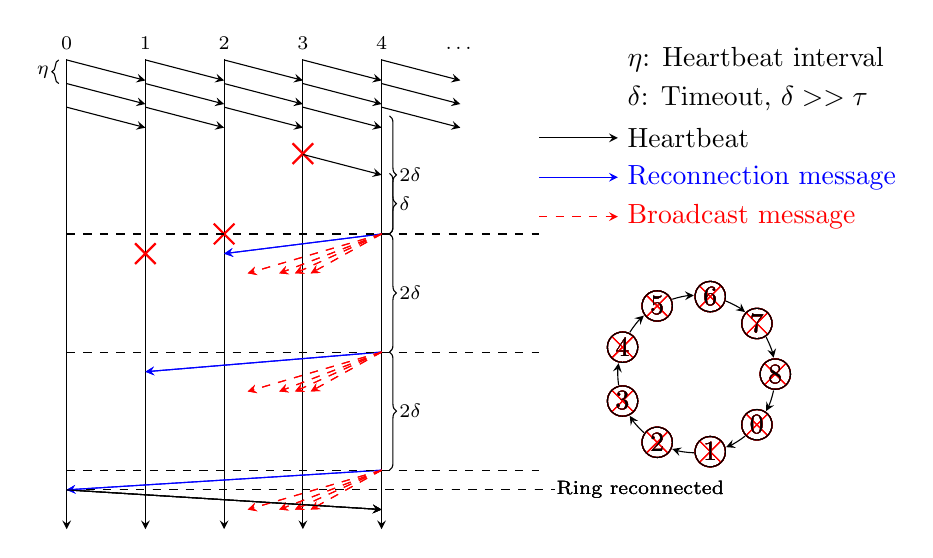
\begin{tikzpicture}[cross/.style={path picture={
  \draw[red]
(path picture bounding box.south east) -- (path picture bounding box.north west) (path picture bounding box.south west) -- (path picture bounding box.north east);
}}]
%%%%% position of the first process and distance between processes
%\begin{minipage}[t]{0.5\textwidth}
\def\z{0}
\def\s{1}
%%%%% lenght of the execution
\def\total{8}
%%%%% delta duration
\def\Tau{0.25}
\def\Eta{0.3}
\def\l{\total-4*\Eta}
\def\Delta{0.75}
%%%failure begin coordinate
\def\fb{0.01}
%%%failure end coordinate
\def\fe{0.50}
%%%% dashed lines for delta
\def\f{0.3}
%%%% number of faults
\def\nbf{3}
\def\propag{0.50}
\pgfmathsetmacro{\nbfmo}{\nbf - 1};
%%%%% beginning of reconnection tentative
\pgfmathsetmacro{\detect}{2 * \Delta}
\def\BeginRec{\l - \fb -\fb - \Tau - \Delta}
\def\Failure3{\BeginRec - \Tau - \Delta - \detect}
\def\EndRec{ \BeginRec - \nbfmo * \detect - \Tau - 2 * \Tau}
%\def\EndRec{\BeginBcast - \nbfmo * \propag - \propag}

%%failure free
  \draw [>=stealth,->] (\z - \s,\total) -- (\z - \s, \EndRec);
  \node at (\z - \s,\total) [font=\scriptsize,above]{$0$};

  \onslide<1-5>{\draw [>=stealth,->] (\z,\total) -- (\z, \EndRec);}
  \node at (\z,\total) [font=\scriptsize,above]{$1$};
\node [right] at (\z + 6, \total) {$\pinginterval$: Heartbeat interval};

\onslide<1-4>{\draw [>=stealth,->] (\z + \s,\total) -- (\z +\s, \EndRec);}
  \node at (\z + \s,\total) [font=\scriptsize,above]{$2$};

\draw [decoration={brace,mirror}, decorate] (\z - \s - 0.10,\total - \fb) -- (\z - \s - 0.10,\total - \fb - \Eta) node [black,midway, 
 left,font=\scriptsize,align=left]{$\pinginterval$};

\onslide<1>{\draw [>=stealth,->] (\z + 2*\s,\total) -- (\z + 2*\s, \EndRec);};
  \node at (\z + 2 * \s, \total) [font=\scriptsize,above]{$3$};

  \draw [>=stealth,->] (\z + 3*\s,\total) -- (\z + 3*\s, \EndRec);
  \node at (\z + 3*\s,\total) [font=\scriptsize,above]{$4$};
  \node at (\z + 4*\s,\total) [font=\scriptsize,above]{\ldots};
\draw [>=stealth,->] (\z + 5, \total - 1) -- (\z + 6, \total - 1) node [right]{Heartbeat};

\foreach \y in {0, 1, 2}
{
\foreach \x in {-1,0,1,2,3}
{  
  \draw  [>=stealth,->] (\z + \x * \s, \total - \fb - \y * \Eta) -- (\z+\x*\s+\s, \total - \fb - \fb - \Tau - \y * \Eta) node [font=\tiny,midway,rotate=331,below]{};
}
}

\onslide<2->{
%% failure of 3

  %  \draw (\z + 2*\s,\total) -- (\z + 2*\s, \l);
  \draw (\z + 2*\s,\total) -- (\z + 2*\s, \total-4*\Eta);
  \draw (\z + 2 * \s,\l) -- (\z + 2 * \s, \l) node [cross out, draw, red,
  thick]{};
  \onslide<3->{\draw [decoration={brace}, decorate] (\z + 3*\s + 0.10,\l - \Tau) -- (\z + 3*\s + 0.10,\BeginRec) node [black,midway, 
  right,font=\scriptsize,align=left]{$\suspectinterval$};}

  \onslide<5->{\draw (\z + \s,\total) -- (\z +\s, \BeginRec) node [cross out, draw, red,
  thick]{};}

\onslide<6->{
\draw (\z,\total) -- (\z,  \BeginRec - \Tau) node [cross out, draw, red,
  thick]{};;}

\draw  [>=stealth,->] (\z + 2*\s, \l - \fb) -- (\z+3*\s, \l - \fb - \fb - \Tau );

\foreach \x in {2,1,0}
{
  \pgfmathtruncatemacro{\y}{2 - \x};
  \pgfmathtruncatemacro{\i}{\x - 1};
  \pgfmathtruncatemacro{\anim}{\y + 3 + 1};

  \ifthenelse{\NOT \x = 0}
             {\onslide<\anim->{\draw [>=stealth,->,blue] (\z + 3 * \s, \BeginRec - \y * \detect) -- (\z + \i * \s, \BeginRec - \Tau - \y * \detect) node [font=\tiny,midway,rotate=15,below]{};
                 \onslide<7>{
                   \foreach \q in {1, 2, 3}
                      {
                        \draw [dashed,red,>=stealth,->] (\z + 3*\s,\BeginRec - \y * \detect) -- (\z + 1.5 *\s + 0.2*\q,\BeginRec - \y * \detect - \propag);
                      }
                      \draw [dashed,red,>=stealth,->] (\z + 3*\s,\BeginRec - \y * \detect) -- (\z + 1.3 *\s,\BeginRec - \y * \detect - \propag);
             }}}
             {\onslide<\anim->{\draw [>=stealth,->,blue] (\z + 3 * \s, \BeginRec - \y * \detect) -- (\z + \i * \s, \BeginRec - \Tau - \y * \detect) node [font=\tiny,midway,rotate=10,above]{};}}
             \pgfmathtruncatemacro{\anime}{\y + 4};
             \onslide<\anime->{\draw[dashed](\z -\s, \BeginRec - \y * \detect) -- (\z + 5*\s,  \BeginRec - \y * \detect);
               \ifthenelse{\y > 0}
                          {\draw [decoration={brace,mirror}, decorate] (\z + 3*\s + 0.10, \BeginRec - \y * \detect) -- (\z + 3*\s + 0.10, \BeginRec - \y * \detect + \detect) node [black,midway, 
                              right,font=\scriptsize,align=left]{2$\suspectinterval$};}{}
             }
             \onslide<\anim->{
               \onslide<7>{
                 \foreach \q in {1, 2, 3}
                    {
                      \draw [dashed,red,>=stealth,->] (\z + 3*\s,\BeginRec - \y * \detect) -- (\z + 1.5 *\s + 0.2*\q,\BeginRec - \y * \detect - \propag);
                    }
                    \draw [dashed,red,>=stealth,->] (\z + 3*\s,\BeginRec - \y * \detect) -- (\z + 1.3 *\s,\BeginRec - \y * \detect - \propag);
             }}
             \ifthenelse{\NOT \x = 0}{}
                        {\onslide<\anim->{
                            \draw [dashed] (-0.75, \BeginRec - \nbfmo * \detect - \Tau) -- (\z + 5 * \s + 0.20, \BeginRec - \nbfmo * \detect - \Tau);
                            \draw (\z + 5*\s + 0.10, \BeginRec - \nbfmo * \detect - \Tau) node [font=\scriptsize,right]{Ring reconnected}; 
%%%heartbeat of the healthy process
                            \draw  [>=stealth,->] (\z-\s, \BeginRec - \nbfmo * \detect - \Tau) -- (\z + 3*\s,  \BeginRec - \nbfmo * \detect - \Tau - \Tau) node [font=\tiny,midway,rotate=350,below]{};}
                        }
}

\onslide<3->{\node [right] at (\z + 6, \total-0.5) {$\suspectinterval$: Timeout, $\suspectinterval >> \msgtime$};}
%\node [left,font=\scriptsize] at (\z + 6, \total-2) {$\msgtime$: Message transmission upper bound};}
\onslide<4->{\draw [>=stealth,->,blue ](\z + 5, \total-1.5) -- (\z + 6, \total-1.5) node [right]{Reconnection message};}
\onslide<7->{\draw [>=stealth,->,dashed,red ](\z + 5, \total-2) -- (\z + 6, \total-2) node [right]{Broadcast message};}

%%% T(3)
%% \draw [dashed] (-0.75, \l - \fb - \fb) -- (3, \l - \fb - \fb);
%% \draw [dashed] (-0.75, \EndRec) -- (3, \EndRec);
%% \draw [>=stealth,<->] (-0.75, \l - \fb - \fb) -- (-0.75, \EndRec) node [font=\scriptsize,left,midway]{$T(\nbf,C)$};

%% \draw (3.25, \EndRec - 0.10) rectangle (6.25,\EndRec - 0.65 - 0.10 - 0.20);
%% \draw node at (3.25, \EndRec - 0.10 - 0.15) [font=\scriptsize,right]{HB=\heartbeat};
%% \draw node at (3.25, \EndRec - 0.10 - 0.40) [font=\scriptsize,right,blue]{NO=\newobserver};
%% \draw node at (3.25, \EndRec - 0.10 - 0.65) [font=\scriptsize,right,red]{Bcast=Broadcast Operation};
}

\def \n {9}
\def \radius {1}
\def \margin {12}
%\node[circle, red, cross,right of=fin] at ({360/\n * 2 - 110}:\radius){7};
%\node[circle, red, cross,right of=fin] at ($(fin.south west)+(3,0)$){6};
\draw node at (\z + 5*\s,  \BeginRec - \detect)(fin){};
%\node(A)[draw,circle,right of=fin,xshift=1cm,yshift=1cm]{0};

\foreach \s in {1,...,\n}
{
  \pgfmathtruncatemacro\id{\n - \s}
  \onslide<1>{
    \node[draw, circle,right of=fin,xshift=6cm,yshift=4cm,inner sep=1pt] at ({360/\n * (\s - 1)}:\radius) {$\id$};
  }
  \onslide<2-4>{
    \ifthenelse{\id = 3}
       {\node[draw,circle, red, cross,right of=fin,xshift=6cm,yshift=4cm,circle,inner sep=1pt] at ({360/\n * (\s - 1)}:\radius){$\id$};}
       {
         \node[draw, circle,right of=fin,xshift=6cm,yshift=4cm,inner sep=1pt] at ({360/\n * (\s - 1)}:\radius) {$\id$};
       }
  }
  \onslide<5>{
    \ifthenelse{\id = 3 \OR \id=2}
             {\node[draw,circle, red, cross,right of=fin,xshift=6cm,yshift=4cm,circle,inner sep=1pt] at ({360/\n * (\s - 1)}:\radius){$\id$};}
             {
               \node[draw, circle,right of=fin,xshift=6cm,yshift=4cm,inner sep=1pt] at ({360/\n * (\s - 1)}:\radius) {$\id$};
             }
  }
  \onslide<6->{
    \ifthenelse{\id = 3 \OR \id=2 \OR \id=1}
               {\node[draw,circle,red,cross,right of=fin,xshift=6cm,yshift=4cm,circle,inner sep=1pt] at ({360/\n * (\s - 1)}:\radius){$\id$};}
               {
                 \node[draw, circle,right of=fin,xshift=6cm,yshift=4cm,inner sep=1pt] at ({360/\n * (\s - 1)}:\radius) {$\id$};
               }
  }
%% \ifthenelse{\s = 6 \OR \s = 7}
  %% {\draw[->, >=stealth,red] ({360/\n * \s -\margin}:\radius)
  %%   arc ({360/\n * \s - \margin}:{360/\n * (\s - 1)+\margin}:\radius);}%|- (\z+5,\total-2)
  \draw[->, >=stealth,xshift=7cm,yshift=4cm] ({360/\n * \s - \margin}:\radius)
    arc ({360/\n * \s - \margin}:{360/\n * (\s - 1) + \margin}:\radius);
}

\end{tikzpicture}
}
\end{overlayarea}
\end{frame}

\begin{frame}
  \frametitle{Failure Notification}

  \begin{columns}
    \begin{column}{0.6\textwidth}
      \begin{itemize}
      \item Hypercube Broadcast Algorithm
        \begin{itemize}
        \item Recursive doubling broadcast algorithm by each node
        \item Completes if $f \leq \lfloor log(n)\rfloor - 1$ ($f$: number of failures, $n$: number of alive processes)
        \item Completes within $2 \tau log(n)$
        \end{itemize}
        \vfill
      \item Application to failure detector
        \begin{itemize}
        \item If $n \neq 2^l$
          \begin{itemize}
          \item $k = \lfloor log(n) \rfloor$ 
          \item $2^k \leq  n  \leq 2^{k+1}$
          \item Initiate two successive broadcast operations
          \end{itemize}
        \item Source $s$ of broadcast sends its current list $D$ of dead processes
        \item {\scriptsize No update of $D$ during broadcast initiated by $s$ -- (do NOT change broadcast topology on the fly)}
        \end{itemize}
      \end{itemize}
    \end{column}

    \begin{column}{0.4\textwidth}
      \centering
      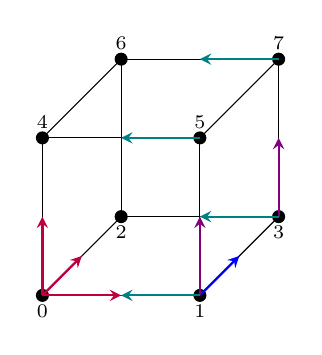
\begin{tikzpicture}
        \def\size{2}
        \def\decalage{1}
        \def\arrowLength{1}
        \foreach \x in {0, 1}
                 {
                   \draw (\x*\decalage,\size+\x*\decalage) -- (\size+\x*\decalage,\size+\x*\decalage);
                   \node [circle,fill=black,scale=0.5] at (\x*\decalage,\size+\x*\decalage){};
                   \pgfmathtruncatemacro{\id}{\x*\decalage*2+4};
                   \node [above,font=\scriptsize] at  (\x*\decalage,\size+\x*\decalage){\id};%{\pgfmathparse{\x*\decalage*2+4}\pgfmathresult};
                   \draw (\x*\decalage,\x*\decalage) -- (\x*\decalage,\size+\x*\decalage);
                   \node [circle,fill=black,scale=0.5] at (\x*\decalage,\x*\decalage){};
                   \pgfmathtruncatemacro{\id}{\x*\decalage*2};
                   \node [below,font=\scriptsize] at (\x*\decalage,\x*\decalage){\id};
                   \draw (\size+\x*\decalage,\size+\x*\decalage) -- (\size+\x*\decalage,\x*\decalage);
                   \node [circle,fill=black,scale=0.5] at (\size+\x*\decalage,\size+\x*\decalage){};
                   \pgfmathtruncatemacro{\id}{\x*\decalage*2+5};
                   \node [above,font=\scriptsize] at (\size+\x*\decalage,\size+\x*\decalage){\id};
                   \draw (\x*\decalage,\x*\decalage) -- (\size+\x*\decalage,\x*\decalage);
                   \node [circle,fill=black,scale=0.5] at (\size+\x*\decalage,\x*\decalage){};
                   \pgfmathtruncatemacro{\id}{\x*\decalage*2+1};
                   \node [below,font=\scriptsize] at (\size+\x*\decalage,\x*\decalage){\id};
                 }
        \draw(0, \size) -- (\decalage, \size+\decalage);
        \draw(\size, \size) -- (\decalage+\size, \size+\decalage);
        \draw(0, 0) -- (\decalage, \decalage);
        \draw(\size, 0) -- (\size+\decalage, \decalage);
        \draw [>=stealth,->,purple,thick] (0,0) -- (\arrowLength,0);
        \draw [>=stealth,->,purple,thick] (0,0) -- (0,\arrowLength);
        \draw [>=stealth,->,purple,thick] (0,0) -- (\arrowLength/2,\arrowLength/2);
        \draw [>=stealth,->,blue,thick] (\size,0) -- (\arrowLength/2+\size,\arrowLength/2);
        \draw [>=stealth,->,violet,thick] (\size,0) -- (\size,\arrowLength);
        \draw [>=stealth,->,violet,thick] (\size+\decalage,\decalage) -- (\size+\decalage,\decalage+\arrowLength);
        \draw [>=stealth,->,teal,thick] (\size,0) -- (\arrowLength,0);
        \draw [>=stealth,->,teal,thick] (\size+\decalage,\decalage) -- (\arrowLength+\decalage,\decalage);
        \draw [>=stealth,->,teal,thick] (\size,\size) -- (\size-\arrowLength,\size);
        \draw [>=stealth,->,teal,thick] (\size+\decalage,\size+\decalage) -- (\size-\arrowLength+\decalage,\size+\decalage);
      \end{tikzpicture}

      \scriptsize
      \begin{tabular}{|c|c|c|c|}
        \hline
        Node & Node1 & Node2 & Node4\\\hline
        1 & \onslide<1->0 & \onslide<1->{0-2-3} &  \onslide<1->{0-4-5}\\
        2 & \onslide<1->{0-1-3} & \onslide<1->0 & \onslide<1->{0-4-6}\\
        3 & \onslide<1->{0-1} & \onslide<1->{0-2} & \onslide<1->{0-4-5-7}\\
        4 & \onslide<1->{0-1-5} & \onslide<1->{0-2-6} & \onslide<1-> 0\\
        5 & \onslide<1->{0-1} & \onslide<1->{0-2-6-7} & \onslide<1->{0-4}\\
        6 & \onslide<1->{0-1-3-7} & \onslide<1->{0-2} & \onslide<1->{0-4}\\
        7 & \onslide<1->{0-1-3} & \onslide<1->{0-2-6} & \onslide<1->{0-4-5}\\\hline
        \end{tabular}
    \end{column}
  \end{columns}

\end{frame}

\begin{frame}
\frametitle{Worst-case analysis}
\begin{center}
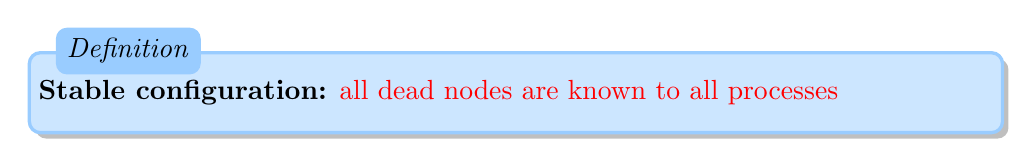
\begin{tikzpicture}
\node [mybox] (box) { %
  \begin{minipage}{1.0\textwidth}
\textbf{Stable configuration:}  \textcolor{red}{all dead nodes are known to all processes}
  \end{minipage}
};
\node [fancytitle, right=10pt] at (box.north west) {\text{\emph{Definition}}};
\end{tikzpicture}
  
\begin{tikzpicture}
\draw [>=stealth,|->](0,5) -- (10,5) node [font=\tiny,below left]{Time}; 
\draw (3,5.10) -- (3,4.90);
\node at (1.50,4.90)[below,font=\scriptsize]{Stable};
\draw (8,5.10) -- (8,4.90);
\node at (9,4.90)[below,font=\scriptsize]{Stable};
\node at (5.5,4.90)[below,font=\scriptsize]{at most $T(f)$ if $f$ faults};
\pic [red] {lightning={3.20,5.5}{3,5}};
%\draw [>=stealth, ->] (3.5, 5.5) -- (3, 5) ;
\pic [red] {lightning={3.70,5.5}{3.5,5}};
\pic [red] {lightning={4.20,5.5}{4,5}};
\node at (3.5,5.5) [above,font=\tiny]{Failures};
\pic [red] {lightning={5.20,5.5}{5,5}};
\pic [red] {lightning={5.70,5.5}{5.5,5}};
\pic [red] {lightning={7.2,5.5}{7,5}};

%\draw [>=stealth,->](0,5) -- (5,10) node [font=\tiny,below left]{Time}; 
\end{tikzpicture}
\end{center}

\begin{theorem}
With $n \leq N$ alive nodes, and for any $f \leq \lfloor \log n \rfloor -1$,
we have
\begin{equation*}
T(f) \leq  f(f+1)  \suspectinterval + f \msgtime + \frac{f(f+1)}{2}(8 \msgtime \log n)
\end{equation*}
\end{theorem}
\begin{itemize}
\item 2 sequential broadcasts: $4 \tau log n$
\item One-port model: broadcast messages and heartbeats interleaved
\end{itemize}

\end{frame}

%% \begin{frame}
%% \frametitle{Worst-case scenario}

%% $$\begin{array}{cccc}
%% T(f) \leq  & \underbrace{f(f+1)  \suspectinterval  +   f \msgtime}  & + &  \underbrace{\frac{f(f+1)}{2}(8 \msgtime \log n)}\\
%% & \textcolor{red}{reconstruction} & & \textcolor{blue}{broadcast}
%% \end{array}$$

%% \begin{itemize}
%% \item $T(f) \leq  \text{ring reconstruction} + \text{broadcasts}$ (for the proof)
%% \item \textcolor{blue}{Process $p$ discovers the death of $q$ at most \textbf{once}\\
%% $\Rightarrow$ $i-th$ dead process discovered dead by at most $f-i+1$ processes\\
%% $\Rightarrow$ at most $\frac{f(f+1)}{2}$ broadcasts}
%% \item \textcolor{red}{$R(f)$ ring reconstruction time\\
%% For $ 1 \leq f \leq \lfloor \log n \rfloor -1$,
%% $$R(f) \leq  R(f-1) + 2f  \suspectinterval + \msgtime$$}
%% \end{itemize}
%% \end{frame}

%% \begin{frame}
%% \frametitle{Ring reconnection}

%% \begin{columns}
%% \begin{column}{0.5\textwidth}

%% $$R(f) \leq  R(f-1) + 2f  \suspectinterval + \msgtime$$

%% \begin{itemize}
%% \item $R(1) \leq 2 \msgtime + \suspectinterval  \leq 2  \suspectinterval + \msgtime$
%% \item $R(f) \leq R(f-1) + R(1)$\\
%% if next failure \emph{non-adjacent}
%% to previous ones
%% \item Worst-case when failing nodes consecutive in the ring
%% \item Build the ring by  \emph{``jumping''} over platform
%% to avoid correlated failures
%% \end{itemize}
%% \end{column}
%% \begin{column}{0.5\textwidth}
%% \scalebox{0.7}{%
%% \begin{tikzpicture}
%% %%%%% position of the first process and distance between processes
%% %\begin{minipage}[t]{0.5\textwidth}
%% \def\z{0}
%% \def\s{0.5}
%% %%%%% lenght of the execution
%% \def\l{6}
%% %%%%% delta duration
%% \def\Tau{0.25}
%% \def\Delta{0.75}
%% %%%failure begin coordinate
%% \def\fb{0.01}
%% %%%failure end coordinate
%% \def\fe{0.50}
%% %%%% dashed lines for delta
%% \def\f{0.3}
%% %%%% number of faults
%% \def\nbf{3}
%% \def\propag{0.50}
%% \pgfmathsetmacro{\nbfmo}{\nbf - 1};
%% %%%%% beginning of reconnection tentative
%% \pgfmathsetmacro{\detect}{2 * \Delta}
%% \def\BeginRec{\l - \fb -\fb - \Tau - \Delta}
%% \def\Failure3{\BeginRec - \Tau - \Delta - \detect}
%% \def\BeginBcast{ \BeginRec - \nbfmo * \detect - \Tau}
%% \def\EndRec{\BeginBcast - \nbfmo * \propag - \propag}
%% %\foreach \x \in {1, 2, 4}
%% %{

%% %}
%% %%   \draw [>=stealth,->] (\z + 4*\s,\l) -- (\z + 4*\s, \EndRec);
%% %%   \node at (\z + 4 * \s,\l) [font=\scriptsize,above]{$5$};

%%   \draw [>=stealth,->] (\z - \s,\l) -- (\z - \s, \EndRec);
%%   \node at (\z - \s,\l) [font=\scriptsize,above]{$0$};

%%   \draw [>=stealth,->] (\z + 3*\s,\l) -- (\z + 3*\s, \EndRec);
%%   \node at (\z + 3*\s,\l) [font=\scriptsize,above]{$4$};
%% %%% nodes
%%   \draw (\z + 2 *\s,\l) -- (\z + 2 * \s, \l) node [cross out, draw, red,
%%   thick]{};
%% %  \node at (\z,\l) [font=\scriptsize,above]{$1$};
%% %\draw (\z + \s,\l) -- (\z + \s, \BeginRec - \Tau - \detect - \Tau - \fb )node [cross out, draw, red,
%%   \draw (\z + \s,\l) -- (\z +\s, \BeginRec) node [cross out, draw, red,
%%   thick]{};
%% \node at (\z + \s,\l) [font=\scriptsize,above]{$2$};
%% \draw (\z,\l) -- (\z,  \BeginRec - \Tau) node [cross out, draw, red,
%%   thick]{};;
%% \node at (\z,\l) [font=\scriptsize,above]{$1$};

%% %\draw (\z, \l) -- (\z, \l - \fb - \fb) node [cross out, draw, red,
%% %  thick]{};
%% \node at (\z + 2 * \s, \l) [font=\scriptsize,above]{$3$};


%% %%%% heartbeat
%% \draw  [>=stealth,->] (\z + 2*\s, \l - \fb) -- (\z+3*\s, \l - \fb - \fb - \Tau ) node [font=\tiny,midway,rotate=331,below]{HB};
%% %%% explanation for failure detection
%% \draw [decoration={brace}, decorate] (\z + 4*\s + 0.5,\l - \fb) -- (\z + 4*\s + 0.5,\BeginRec) node [black,midway,
%%   right,font=\scriptsize,align=left]{$\msgtime + \suspectinterval \leq 2 \suspectinterval$ to detect the \\ failure of $3$};


%% %%%%% Failures detection of 2 delimitation
%% %\draw[dashed](\z -\s, \BeginRec - \Tau - \Delta) -- (\z + 5*\s,  \BeginRec - \Tau - \Delta);
%% %\draw [decoration={brace}, decorate] (\z + 4*\s + 0.25, \BeginRec) -- (\z + 4*\s + 0.25,\BeginRec - \Tau - \Delta) node [black,midway,
%% %  right,font=\tiny,align=left]{$3$ detects failure of $2$ after $R(1)$\\ This failure increases the size \\ of the segment $I_1=\{1\}$ by one};



%% %%%% 4 detects 3's failure
%% %\draw [decoration={brace}, decorate] (\z + 4*\s + 0.25, \Failure3) -- (\z + 4*\s + 0.25,\Failure3 - \Tau - \Delta) node [black,midway,
%% %  right,font=\tiny,align=left]{$4$ detects failure of $3$ after $R(1)$\\ This failure increases the size of \\ the segment $I_1=\{1,2\}$ by one};


%% %%%% 4's reconnection messages
%% \foreach \x in {2,1,0}
%% {
%%   \pgfmathtruncatemacro{\y}{2 - \x};
%%   \pgfmathtruncatemacro{\i}{\x - 1};
%%   \ifthenelse{\NOT \x = 0}
%%              {\draw [>=stealth,->,blue] (\z + 3 * \s, \BeginRec - \y * \detect) -- (\z + \i * \s, \BeginRec - \Tau - \y * \detect) node [font=\tiny,midway,rotate=15,below]{NO};}
%%              {\draw [>=stealth,->,blue] (\z + 3 * \s, \BeginRec - \y * \detect) -- (\z + \i * \s, \BeginRec - \Tau - \y * \detect) node [font=\tiny,midway,rotate=10,above]{NO};}
%%   \draw[dashed](\z -\s, \BeginRec - \y * \detect) -- (\z + 5*\s,  \BeginRec - \y * \detect);
%% \ifthenelse{\NOT \x = 0}{
%% \ifthenelse{\x = 2}{
%%   \draw [decoration={brace}, decorate] (\z + 4*\s + 0.25, \BeginRec - \y * \detect) -- (\z + 4*\s + 0.25,\BeginRec - \y * \detect - \detect) node [black,midway,
%%  right,font=\scriptsize,align=left]{$4$ detects failure of $\x$ after $2\suspectinterval$};}
%% {
%%   \draw [decoration={brace}, decorate] (\z + 4*\s + 0.25, \BeginRec - \y * \detect) -- (\z + 4*\s + 0.25,\BeginRec - \y * \detect - \detect) node [black,midway,
%%  right,font=\scriptsize,align=left]{$4$ detects failure of $\x$ after $2\suspectinterval$};}
%% }
%% {
%% \draw [dashed] (-0.75, \BeginRec - \nbfmo * \detect - \Tau) -- (\z + 5 * \s + 0.20, \BeginRec - \nbfmo * \detect - \Tau);
%% \draw (\z + 5*\s + 0.10, \BeginRec - \nbfmo * \detect - \Tau) node [font=\scriptsize,right]{Ring reconnected};
%% %%%heartbeat of the healthy process
%% \draw  [>=stealth,->] (\z-\s, \BeginRec - \nbfmo * \detect - \Tau) -- (\z + 3*\s,  \BeginRec - \nbfmo * \detect - \Tau - \Tau) node [font=\tiny,midway,rotate=350,below]{HB};
%% }
%% }


%% %%%% Broadcast begin
%% \foreach \x in {1,...,\nbf}
%% {
%%   \pgfmathtruncatemacro{\y}{\x - 1};
%%   \pgfmathtruncatemacro{\p}{4 - \x};
%% \foreach \q in {1, 2, 3}
%% {
%%   \draw [dashed,red,>=stealth,->] (\z + 3*\s,\BeginBcast - \y * \propag) -- (\z + 1.5 *\s + 0.2*\q,\BeginBcast - \y * \propag - \propag);
%% }

%% %\ifthenelse{\x = 2}
%% %{  \draw [dashed,red,>=stealth,->] (\z + 3*\s,\BeginBcast - \y * \propag) -- (\z + 1.3 *\s,\BeginBcast - \y * \propag - \propag);
%%  \draw [dashed,red,>=stealth,->] (\z + 3*\s,\BeginBcast - \y * \propag) -- (\z + 1.3 *\s,\BeginBcast - \y * \propag - \propag);
%%   \draw [decoration={brace}, decorate] (\z + 3 *\s + 0.10,\BeginBcast - \y * \propag) -- (\z + 3*\s + 0.10,\BeginBcast - \propag - \y * \propag) node [black,midway,
%%   right,font=\tiny,align=left]{$8 \msgtime \log n$};
%% }

%% \draw node at (\z + 1.3 *\s,\BeginBcast -  \propag - \propag  + 0.10) [font=\tiny,left,red]{Bcast};

%% \draw [decoration={brace}, decorate,white] (\z + 3 *\s + 1,\BeginBcast) -- (\z + 3*\s + 1,\BeginBcast -  \nbf * \propag) node [black,midway,
%%   right,font=\scriptsize,align=left]{Broadcast messages of the \\ failure of processes $3$, $2$ and $1$};

%% %%% T(3)
%% \draw [dashed] (-0.75, \l - \fb - \fb) -- (3, \l - \fb - \fb);
%% \draw [dashed] (-0.75, \EndRec) -- (3, \EndRec);
%% \draw [>=stealth,<->] (-0.75, \l - \fb - \fb) -- (-0.75, \EndRec) node [font=\scriptsize,left,midway]{$T(\nbf,C)$};

%% \draw (3.25, \EndRec - 0.10) rectangle (6.60,\EndRec - 0.65 - 0.10 - 0.20);
%% \draw node at (3.25, \EndRec - 0.10 - 0.15) [font=\scriptsize,right]{HB=\heartbeat};
%% \draw node at (3.25, \EndRec - 0.10 - 0.40) [font=\scriptsize,right,blue]{NO=\newobserver};
%% \draw node at (3.25, \EndRec - 0.10 - 0.65) [font=\scriptsize,right,red]{Bcast=Broadcast Operation};

%% %\draw[dashed](0, \l - \fb) -- (5, \l - \fb);

%% %% \foreach \x in {1,3}
%% %% {
%% %%   \pgfmathtruncatemacro{\y}{3 - \x};
%% %%   \draw[dashed](\z -\s, \BeginRec - \y * \detect - \y * \Tau) -- (\z + 5*\s,  \BeginRec - \y * \detect - \y * \Tau);
%% %% }
%% %% \draw[dashed](\z -\s, \BeginRec - 3 * \detect - 2 * \Tau) -- (\z + 5*\s,  \BeginRec - 3 * \detect - 2 * \Tau);

%% \end{tikzpicture}
%% }
%% \end{column}
%% \end{columns}
%% \end{frame}

%% \begin{frame}
%% \frametitle{Noise}
%% \hspace*{-0.5cm}
%% 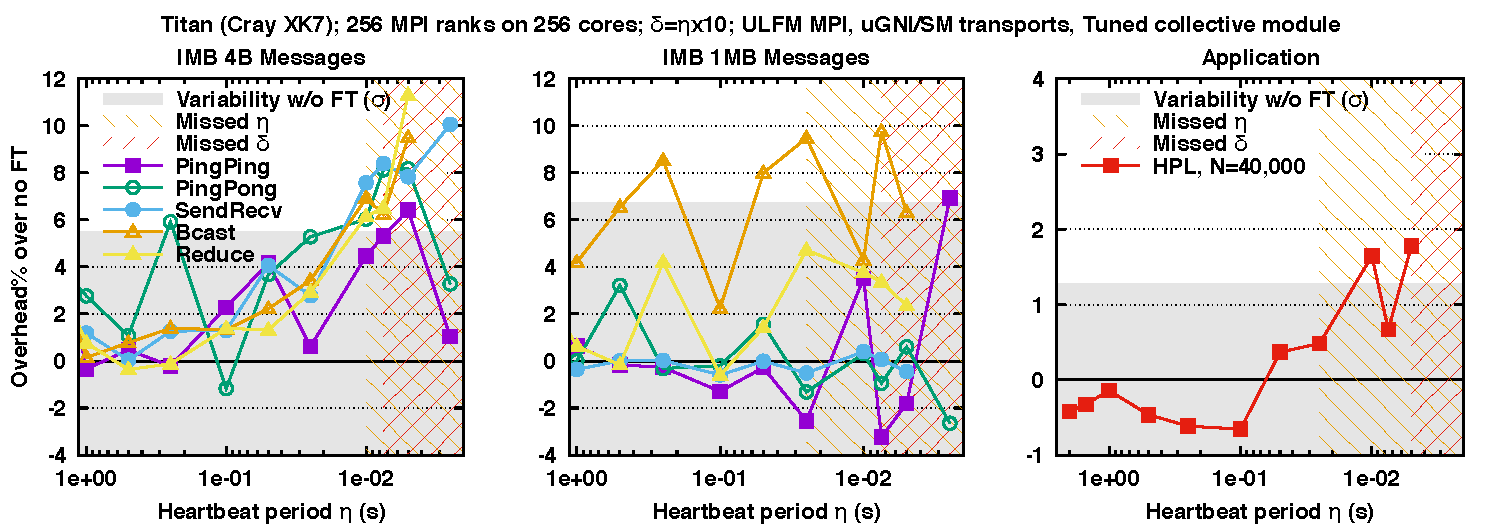
\includegraphics[width=1.1\textwidth]{etanoise-titan.pdf}
%% \end{frame}

\begin{frame}
\frametitle{Detection and propagation delay}
\hspace*{-0.5cm}
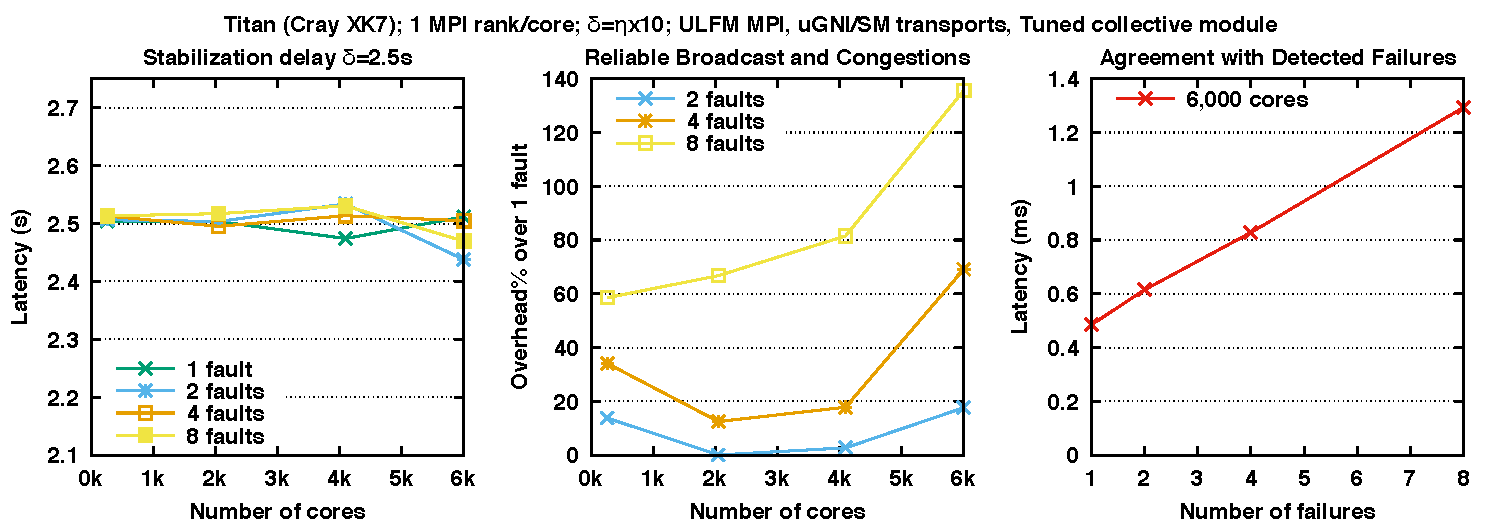
\includegraphics[width=1.1\textwidth]{recva-titan.pdf}
\end{frame}

\begin{frame}
  \frametitle{Algorithm-Based Fault Tolerant LU over ULFM}

  \begin{columns}
    \begin{column}{.3\textwidth}
      \begin{itemize}
      \item Algorithm-Based Fault Tolerant LU (PDGETRF) based on ULFM
        \begin{itemize}
        \item Replication to ensure checksum availability
        \item Partial checkpoint to rollback Q-panel operation
        \item ABFT to recover most of the missing data
        \item Partial re-execution to recover panel
        \end{itemize}
      \end{itemize}
    \end{column}
    \begin{column}{.7\textwidth}
        \begin{center}
          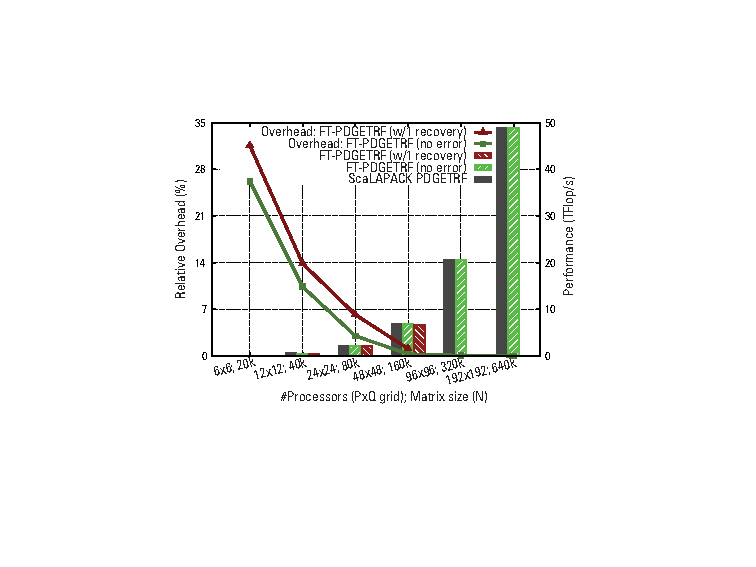
\includegraphics[width=.9\linewidth]{abftlu-perf.pdf}
        \end{center}
    \end{column}
  \end{columns}
\end{frame}


\begin{frame}
  \frametitle{Conclusion on Application-Specific Fault Tolerance}

  \begin{itemize}
  \item Many applications are amenable to 'Roll-Forward' approaches
    \begin{itemize}
    \item No Re-Execution, no TLost! (or very little)
    \end{itemize}
  \item Performance of roll-forward is orders of magnitude higher than checkpoint/restart
    \begin{itemize}
    \item And it scales better!
    \end{itemize}
  \item Roll-forward is only for specific parts of real life applications
    \begin{itemize}
    \item But we have composition techniques!
    \end{itemize}
  \item Roll-forward requires a resilient communication middleware
    \begin{itemize}
    \item ULFM is integrated in Open MPI and MPICH
    \item Overhead on failure-free is non measurable
    \item Overhead on failure-specific operation is very small
    \item It is slowly being integrated in the MPI Standard
    \end{itemize}
  \end{itemize}
  
\end{frame}

\section[Major Contribution 2]{Major Contribution 2: Distributed-memory multi-GPU block-sparse tensor contraction for electronic structure}

\begin{frame}[t]
  \frametitle{Electronic Structure Application}

  \begin{itemize}
  \item Accurate simulation of electronic structure
  \item Quantum Chemistry
  \item Coupled Cluster Singles and Doubles (CCSD)
    \begin{itemize}
    \item $O(n^6)$, $O(n^4)$ space. $n = O(\textrm{\# atoms})$
    \item $\Rightarrow$ a few (5-10) atoms on a workstation
    \item a few dozen (50-100) atoms on a supercomputer
    \end{itemize}
  \item fast/reduced scaling formulations $\Rightarrow$ 100s of atoms on a workstation
    \begin{itemize}
    \item Time to solution in days
    \item \textcolor{teal}{$\Rightarrow$ we should get time to solutions in minutes on a supercomputer}
    \end{itemize}
  \item Complex tensor algebra
  \item Single terms represents 90\% of computation:
  \end{itemize}

  $$
  R_{ab}^{ij} = \sum_{cd} T_{cd}^{ij}V_{ab}^{cd} + \ldots
  $$
  
\end{frame}

%% \begin{frame}[t]
%%   \frametitle{ABCD tensor product}

%%   \begin{center}
%%   \begin{tikzpicture}
%%     \node at (0,0) {$
%%       \tikzmarknode{R}{R}_{\tikzmarknode{ab}{ab}}^{\tikzmarknode{ij}{ij}} = \sum_{\tikzmarknode{cd}{cd}}
%%       \tikzmarknode{T}{T_{cd}^{ij}}\tikzmarknode{V}{V_{ab}^{cd}} + \ldots
%%       $};
%%     \draw[teal,-latex,line width=.5mm] (1,-2) node[below,teal] {Elements to be refined iteratively (typically 10-20 iterations)} .. controls (1,-1) and ([yshift=-1cm]T.south) .. (T.south);
%%     \draw[teal,-latex,line width=.5mm] (2.5,2) node[above,teal] {Fixed between iterations} .. controls (2.5,1) and ([yshift=1cm]V.north) .. (V.north);
%%     \draw[teal,-latex,line width=.5mm] (-3,0) node[left,teal] {Make vanish} -- (R.west);
%%     \draw[orange,-latex,line width=.5mm] (-2.5,1) node[above,orange] {M} .. controls (-2.5,0.5) and ([yshift=0.5cm]ij.north) .. (ij.north);
%%     \draw[orange,-latex,line width=.5mm] (-2.5,-1) node[below,orange] {N} .. controls (-2.5,-0.5) and ([yshift=-0.5cm]ab.south) .. (ab.south);
%%     \draw[orange,-latex,line width=.5mm] (-1,-1.25) node[below,orange] {K} .. controls (-1,-0.5) and ([yshift=-0.5cm]cd.south) .. (cd.south);
%%   \end{tikzpicture}
%%   \end{center}

%%   \begin{tikzpicture}[remember picture,overlay]
%%     \node[orange,xshift=-4cm,yshift=1.5cm,align=center] at (current page.south east) {
%%       $C_{m,n} \leftarrow C_{m,n} + A_{m, k}B_{k, n}$,\\
%%       with $m\in [1, M], n\in [1, N], k\in [1, K]$\\
%%       and $N = K >> M$};
%%   \end{tikzpicture}

%%   \begin{itemize}
%%   \item $i, j, a, b, c, d = O(n)$
%%   \item $i = j, a = b = c = d = [5, 20]i$
%%   \end{itemize}
%% \end{frame}

\begin{frame}[t]
  \frametitle{Block-Sparse Representation}

  \begin{columns}
    \begin{column}{0.5\textwidth}
    \resizebox{8cm}{!}{\begin{tikzpicture}[
        %Global config
        baseline=0cm,
        >={Stealth[length=7pt,width=13pt]},
        line width=.5pt,
        ampersand replacement=\&,
        %Styles
        Matrix/.style={
            matrix of nodes,
            font=\scriptsize,
            text height=1.5pt,
            text depth=1pt,
            text width=1.5pt,
            align=center,
            column sep=1.5pt,
            row sep=1.5pt,
            nodes in empty cells,
        },
    ]

    \matrix[Matrix] at (0,0) (B){ % Matrix contents 
        \& \& \& \& \& \& \& \& \& \&  \\
        \& \& \& \& \& \& \& \& \& \&\\
        \& \& \& \& \& \& \& \& \& \&  \\
        \& \& \& \& \& \& \& \& \& \&\\
        \& \& \& \& \& \& \& \& \& \&  \\
        \& \& \& \& \& \& \& \& \& \&\\
        \& \& \& \& \& \& \& \& \& \&  \\
        \& \& \& \& \& \& \& \& \& \&\\
        \& \& \& \& \& \& \& \& \& \&  \\
        \& \& \& \& \& \& \& \& \& \&\\
        \& \& \& \& \& \& \& \& \& \&  \\
    };

    \matrix[Matrix,below=2pt of B.south] (C){ % Matrix contents 
        \& \& \& \& \& \& \& \& \& \&\\
        \& \& \& \& \& \& \& \& \& \&\\
        \& \& \& \& \& \& \& \& \& \&\\
        \& \& \& \& \& \& \& \& \& \&\\
        \& \& \& \& \& \& \& \& \& \&\\
        \& \& \& \& \& \& \& \& \& \&\\
   };

    \matrix[Matrix,left=2pt of C.west] (A){ % Matrix contents 
        \& \& \& \& \& \& \& \& \& \&\\
        \& \& \& \& \& \& \& \& \& \&\\
        \& \& \& \& \& \& \& \& \& \&\\
        \& \& \& \& \& \& \& \& \& \&\\
        \& \& \& \& \& \& \& \& \& \&\\
        \& \& \& \& \& \& \& \& \& \&\\
   };

   \node[draw,fill=gray!25,inner sep=0,fit=(A-1-1)(A-1-1)](A00){};
   \node[draw,inner sep=0,fit=(A-2-1)(A-2-1)](A10){};
   \node[draw,fill=gray!25,inner sep=0,fit=(A-3-1)(A-4-1)](A20){};
   \node[draw,inner sep=0,fit=(A-5-1)(A-5-1)](A30){};
   \node[draw,fill=gray!25,inner sep=0,fit=(A-6-1)(A-6-1)](A40){};

   \node[draw,inner sep=0,fit=(A-1-2)(A-1-3)](A01){};
   \node[draw,fill=gray!25,inner sep=0,fit=(A-2-2)(A-2-3)](A11){};
   \node[draw,fill=gray!25,inner sep=0,fit=(A-3-2)(A-4-3)](A21){};
   \node[draw,fill=gray!25,inner sep=0,fit=(A-5-2)(A-5-3)](A31){};
   \node[draw,inner sep=0,fit=(A-6-2)(A-6-3)](A41){};

   \node[draw,fill=gray!25,inner sep=0,fit=(A-1-4)(A-1-6)](A02){};
   \node[draw,inner sep=0,fit=(A-2-4)(A-2-6)](A12){};
   \node[draw,fill=gray!25,inner sep=0,fit=(A-3-4)(A-4-6)](A22){};
   \node[draw,inner sep=0,fit=(A-5-4)(A-5-6)](A32){};
   \node[draw,inner sep=0,fit=(A-6-4)(A-6-6)](A42){};

   \node[draw,fill=gray!25,inner sep=0,fit=(A-1-7)(A-1-9)](A03){};
   \node[draw,fill=gray!25,inner sep=0,fit=(A-2-7)(A-2-9)](A13){};
   \node[draw,fill=gray!25,inner sep=0,fit=(A-3-7)(A-4-9)](A23){};
   \node[draw,fill=gray!25,inner sep=0,fit=(A-5-7)(A-5-9)](A33){};
   \node[draw,inner sep=0,fit=(A-6-7)(A-6-9)](A43){};

   \node[draw,inner sep=0,fit=(A-1-10)(A-1-10)](A04){};
   \node[draw,fill=gray!25,inner sep=0,fit=(A-2-10)(A-2-10)](A14){};
   \node[draw,fill=gray!25,inner sep=0,fit=(A-3-10)(A-4-10)](A24){};
   \node[draw,inner sep=0,fit=(A-5-10)(A-5-10)](A34){};
   \node[draw,fill=gray!25,inner sep=0,fit=(A-6-10)(A-6-10)](A44){};

   \node[draw,fill=gray!25,inner sep=0,fit=(A-1-11)(A-1-11)](A05){};
   \node[draw,inner sep=0,fit=(A-2-11)(A-2-11)](A15){};
   \node[draw,inner sep=0,fit=(A-3-11)(A-4-11)](A25){};
   \node[draw,fill=gray!25,inner sep=0,fit=(A-5-11)(A-5-11)](A35){};
   \node[draw,inner sep=0,fit=(A-6-11)(A-6-11)](A45){};

   \node[draw,fill=gray!25,inner sep=0,fit=(B-1-1)(B-1-2)](B00){};
   \node[draw,inner sep=0,fit=(B-2-1)(B-3-2)](B10){};
   \node[draw,fill=gray!25,inner sep=0,fit=(B-4-1)(B-6-2)](B20){};
   \node[draw,fill=gray!25,inner sep=0,fit=(B-7-1)(B-9-2)](B30){};
   \node[draw,inner sep=0,fit=(B-10-1)(B-10-2)](B40){};
   \node[draw,fill=gray!25,inner sep=0,fit=(B-11-1)(B-11-2)](B50){};

   \node[draw,inner sep=0,fit=(B-1-3)(B-1-5)](B01){};
   \node[draw,fill=gray!25,inner sep=0,fit=(B-2-3)(B-3-5)](B11){};
   \node[draw,inner sep=0,fit=(B-4-3)(B-6-5)](B21){};
   \node[draw,inner sep=0,fit=(B-7-3)(B-9-5)](B31){};
   \node[draw,fill=gray!25,inner sep=0,fit=(B-10-3)(B-10-5)](B41){};
   \node[draw,inner sep=0,fit=(B-11-3)(B-11-5)](B51){};

   \node[draw,inner sep=0,fit=(B-1-6)(B-1-7)](B02){};
   \node[draw,inner sep=0,fit=(B-2-6)(B-3-7)](B12){};
   \node[draw,fill=gray!25,inner sep=0,fit=(B-4-6)(B-6-7)](B22){};
   \node[draw,inner sep=0,fit=(B-7-6)(B-9-7)](B32){};
   \node[draw,fill=gray!25,inner sep=0,fit=(B-10-6)(B-10-7)](B42){};
   \node[draw,inner sep=0,fit=(B-11-6)(B-11-7)](B52){};

   \node[draw,inner sep=0,fit=(B-1-8)(B-1-9)](B03){};
   \node[draw,fill=gray!25,inner sep=0,fit=(B-2-8)(B-3-9)](B13){};
   \node[draw,inner sep=0,fit=(B-4-8)(B-6-9)](B23){};
   \node[draw,inner sep=0,fit=(B-7-8)(B-9-9)](B33){};
   \node[draw,fill=gray!25,inner sep=0,fit=(B-10-8)(B-10-9)](B43){};
   \node[draw,inner sep=0,fit=(B-11-8)(B-11-9)](B53){};

   \node[draw,inner sep=0,fit=(B-1-10)(B-1-10)](B04){};
   \node[draw,fill=gray!25,inner sep=0,fit=(B-2-10)(B-3-10)](B14){};
   \node[draw,fill=gray!25,inner sep=0,fit=(B-4-10)(B-6-10)](B24){};
   \node[draw,fill=gray!25,inner sep=0,fit=(B-7-10)(B-9-10)](B34){};
   \node[draw,inner sep=0,fit=(B-10-10)(B-10-10)](B44){};
   \node[draw,inner sep=0,fit=(B-11-10)(B-11-10)](B54){};

   \node[draw,fill=gray!25,inner sep=0,fit=(B-1-11)(B-1-11)](B05){};
   \node[draw,inner sep=0,fit=(B-2-11)(B-3-11)](B15){};
   \node[draw,fill=gray!25,inner sep=0,fit=(B-4-11)(B-6-11)](B25){};
   \node[draw,inner sep=0,fit=(B-7-11)(B-9-11)](B35){};
   \node[draw,inner sep=0,fit=(B-10-11)(B-10-11)](B45){};
   \node[draw,inner sep=0,fit=(B-11-11)(B-11-11)](B55){};

   \node[draw,fill=gray!25,inner sep=0,fit=(C-1-1)(C-1-2)](C00){};
   \node[draw,inner sep=0,fit=(C-2-1)(C-2-2)](C10){};
   \node[draw,fill=gray!25,inner sep=0,fit=(C-3-1)(C-4-2)](C20){};
   \node[draw,fill=gray!25,inner sep=0,fit=(C-5-1)(C-5-2)](C30){};
   \node[draw,fill=gray!25,inner sep=0,fit=(C-6-1)(C-6-2)](C40){};

   \node[draw,inner sep=0,fit=(C-1-3)(C-1-5)](C01){};
   \node[draw,fill=gray!25,inner sep=0,fit=(C-2-3)(C-2-5)](C11){};
   \node[draw,fill=gray!25,inner sep=0,fit=(C-3-3)(C-4-5)](C21){};
   \node[draw,fill=gray!25,inner sep=0,fit=(C-5-3)(C-5-5)](C31){};
   \node[draw,inner sep=0,fit=(C-6-3)(C-6-5)](C41){};

   \node[draw,fill=gray!25,inner sep=0,fit=(C-1-6)(C-1-7)](C02){};
   \node[draw,fill=gray!25,inner sep=0,fit=(C-2-6)(C-2-7)](C12){};
   \node[draw,fill=gray!25,inner sep=0,fit=(C-3-6)(C-4-7)](C22){};
   \node[draw,inner sep=0,fit=(C-5-6)(C-5-7)](C32){};
   \node[draw,fill=gray!25,inner sep=0,fit=(C-6-6)(C-6-7)](C42){};

   \node[draw,inner sep=0,fit=(C-1-8)(C-1-9)](C03){};
   \node[draw,fill=gray!25,inner sep=0,fit=(C-2-8)(C-2-9)](C13){};
   \node[draw,fill=gray!25,inner sep=0,fit=(C-3-8)(C-4-9)](C23){};
   \node[draw,fill=gray!25,inner sep=0,fit=(C-5-8)(C-5-9)](C33){};
   \node[draw,fill=gray!25,inner sep=0,fit=(C-6-8)(C-6-9)](C43){};

   \node[draw,fill=gray!25,inner sep=0,fit=(C-1-10)(C-1-10)](C04){};
   \node[draw,fill=gray!25,inner sep=0,fit=(C-2-10)(C-2-10)](C14){};
   \node[draw,fill=gray!25,inner sep=0,fit=(C-3-10)(C-4-10)](C24){};
   \node[draw,fill=gray!25,inner sep=0,fit=(C-5-10)(C-5-10)](C34){};
   \node[draw,inner sep=0,fit=(C-6-10)(C-6-10)](C44){};

   \node[draw,fill=gray!25,inner sep=0,fit=(C-1-11)(C-1-11)](C05){};
   \node[draw,inner sep=0,fit=(C-2-11)(C-2-11)](C15){};
   \node[draw,fill=gray!25,inner sep=0,fit=(C-3-11)(C-4-11)](C25){};
   \node[draw,inner sep=0,fit=(C-5-11)(C-5-11)](C35){};
   \node[draw,fill=gray!25,inner sep=0,fit=(C-6-11)(C-6-11)](C45){};

   \path[left] (A00.north west) -- node (l2) {$p_0$} (A00.south west);
   \path[left] (A10.north west) -- node {$p_1$} (A10.south west);
   \path[left] (A20.north west) -- node {$p_0$} (A20.south west);
   \path[left] (A30.north west) -- node {$p_1$} (A30.south west);
   \path[left] (A40.north west) -- node (l3) {$p_0$} (A40.south west);

   \path[above] (A00.north west) -- node (l4) {$q_0$} (A00.north east);
   \path[above] (A01.north west) -- node {$q_1$} (A01.north east);
   \path[above] (A02.north west) -- node {$q_0$} (A02.north east);
   \path[above] (A03.north west) -- node {$q_1$} (A03.north east);
   \path[above] (A04.north west) -- node {$q_0$} (A04.north east);
   \path[above] (A05.north west) -- node (l6) {$q_1$} (A05.north east);

   \draw [decorate,decoration={brace,amplitude=5pt},above] (l4.north west) -- (l6.north east) node [black,midway,yshift=3pt] {\footnotesize $A$ is distributed 2D cyclic};

    \end{tikzpicture}}
    \end{column}

    \begin{column}{.5\textwidth}
      \relsize{-1}
      \begin{itemize}
      \item Tiling is non-uniform, motivated by the physics
      \item Cannot tile evenly without sacrificing locality
      \item Blocks can be empty
      \item Density can range form quite sparse (2\%) to quite dense (30\%)
      \item $B$ is huge: may not fit in distributed memory
        \begin{itemize}
        \item Tiles of $B$ can be generated on demand
        \item Generation of a tile is $\geq O(nb\times mb)$ and may
          require comm.
        \end{itemize}
      \item $A$, $B$ or $C$ may not fit on the (accumulated) GPU memory
      \end{itemize}
    \end{column}
    \end{columns}
  
\end{frame}


\begin{frame}[t]
  \frametitle{Design Principles (distributed)}

  \begin{columns}
    \begin{column}{0.5\textwidth}
    \resizebox{8cm}{!}{\begin{tikzpicture}[
        %Global config
        baseline=0cm,
        >={Stealth[length=7pt,width=13pt]},
        line width=.5pt,
        ampersand replacement=\&,
        %Styles
        Matrix/.style={
            matrix of nodes,
            font=\scriptsize,
            text height=1.5pt,
            text depth=1pt,
            text width=1.5pt,
            align=center,
            column sep=1.5pt,
            row sep=1.5pt,
            nodes in empty cells,
        },
    ]

    \matrix[Matrix] at (0,0) (B){ % Matrix contents 
        \& \& \& \& \& \& \& \& \& \&  \\
        \& \& \& \& \& \& \& \& \& \&\\
        \& \& \& \& \& \& \& \& \& \&  \\
        \& \& \& \& \& \& \& \& \& \&\\
        \& \& \& \& \& \& \& \& \& \&  \\
        \& \& \& \& \& \& \& \& \& \&\\
        \& \& \& \& \& \& \& \& \& \&  \\
        \& \& \& \& \& \& \& \& \& \&\\
        \& \& \& \& \& \& \& \& \& \&  \\
        \& \& \& \& \& \& \& \& \& \&\\
        \& \& \& \& \& \& \& \& \& \&  \\
    };

    \matrix[Matrix,below=2pt of B.south] (C){ % Matrix contents 
        \& \& \& \& \& \& \& \& \& \&\\
        \& \& \& \& \& \& \& \& \& \&\\
        \& \& \& \& \& \& \& \& \& \&\\
        \& \& \& \& \& \& \& \& \& \&\\
        \& \& \& \& \& \& \& \& \& \&\\
        \& \& \& \& \& \& \& \& \& \&\\
   };

    \matrix[Matrix,left=2pt of C.west] (A){ % Matrix contents 
        \& \& \& \& \& \& \& \& \& \&\\
        \& \& \& \& \& \& \& \& \& \&\\
        \& \& \& \& \& \& \& \& \& \&\\
        \& \& \& \& \& \& \& \& \& \&\\
        \& \& \& \& \& \& \& \& \& \&\\
        \& \& \& \& \& \& \& \& \& \&\\
   };

   \node[draw,fill=gray!75,inner sep=0,fit=(A-1-1)(A-1-1)](A00){};
   \node[draw,inner sep=0,fit=(A-2-1)(A-2-1)](A10){};
   \node[draw,fill=gray!75,inner sep=0,fit=(A-3-1)(A-4-1)](A20){};
   \node[draw,inner sep=0,fit=(A-5-1)(A-5-1)](A30){};
   \node[draw,fill=gray!75,inner sep=0,fit=(A-6-1)(A-6-1)](A40){};

   \node[draw,inner sep=0,fit=(A-1-2)(A-1-3)](A01){};
   \node[draw,fill=gray!25,inner sep=0,fit=(A-2-2)(A-2-3)](A11){};
   \node[draw,fill=gray!75,inner sep=0,fit=(A-3-2)(A-4-3)](A21){};
   \node[draw,fill=gray!25,inner sep=0,fit=(A-5-2)(A-5-3)](A31){};
   \node[draw,inner sep=0,fit=(A-6-2)(A-6-3)](A41){};

   \node[draw,fill=gray!75,inner sep=0,fit=(A-1-4)(A-1-6)](A02){};
   \node[draw,inner sep=0,fit=(A-2-4)(A-2-6)](A12){};
   \node[draw,fill=gray!75,inner sep=0,fit=(A-3-4)(A-4-6)](A22){};
   \node[draw,inner sep=0,fit=(A-5-4)(A-5-6)](A32){};
   \node[draw,inner sep=0,fit=(A-6-4)(A-6-6)](A42){};

   \node[draw,fill=gray!75,inner sep=0,fit=(A-1-7)(A-1-9)](A03){};
   \node[draw,fill=gray!25,inner sep=0,fit=(A-2-7)(A-2-9)](A13){};
   \node[draw,fill=gray!75,inner sep=0,fit=(A-3-7)(A-4-9)](A23){};
   \node[draw,fill=gray!25,inner sep=0,fit=(A-5-7)(A-5-9)](A33){};
   \node[draw,inner sep=0,fit=(A-6-7)(A-6-9)](A43){};

   \node[draw,inner sep=0,fit=(A-1-10)(A-1-10)](A04){};
   \node[draw,fill=gray!25,inner sep=0,fit=(A-2-10)(A-2-10)](A14){};
   \node[draw,fill=gray!75,inner sep=0,fit=(A-3-10)(A-4-10)](A24){};
   \node[draw,inner sep=0,fit=(A-5-10)(A-5-10)](A34){};
   \node[draw,fill=gray!75,inner sep=0,fit=(A-6-10)(A-6-10)](A44){};

   \node[draw,fill=gray!75,inner sep=0,fit=(A-1-11)(A-1-11)](A05){};
   \node[draw,inner sep=0,fit=(A-2-11)(A-2-11)](A15){};
   \node[draw,inner sep=0,fit=(A-3-11)(A-4-11)](A25){};
   \node[draw,fill=gray!25,inner sep=0,fit=(A-5-11)(A-5-11)](A35){};
   \node[draw,inner sep=0,fit=(A-6-11)(A-6-11)](A45){};

   \node[draw,fill=gray!75,inner sep=0,fit=(B-1-1)(B-1-2)](B00){};
   \node[draw,inner sep=0,fit=(B-2-1)(B-3-2)](B10){};
   \node[draw,fill=gray!75,inner sep=0,fit=(B-4-1)(B-6-2)](B20){};
   \node[draw,fill=gray!75,inner sep=0,fit=(B-7-1)(B-9-2)](B30){};
   \node[draw,inner sep=0,fit=(B-10-1)(B-10-2)](B40){};
   \node[draw,fill=gray!75,inner sep=0,fit=(B-11-1)(B-11-2)](B50){};

   \node[draw,inner sep=0,fit=(B-1-3)(B-1-5)](B01){};
   \node[draw,fill=gray!25,inner sep=0,fit=(B-2-3)(B-3-5)](B11){};
   \node[draw,inner sep=0,fit=(B-4-3)(B-6-5)](B21){};
   \node[draw,inner sep=0,fit=(B-7-3)(B-9-5)](B31){};
   \node[draw,fill=gray!25,inner sep=0,fit=(B-10-3)(B-10-5)](B41){};
   \node[draw,inner sep=0,fit=(B-11-3)(B-11-5)](B51){};

   \node[draw,inner sep=0,fit=(B-1-6)(B-1-7)](B02){};
   \node[draw,inner sep=0,fit=(B-2-6)(B-3-7)](B12){};
   \node[draw,fill=gray!25,inner sep=0,fit=(B-4-6)(B-6-7)](B22){};
   \node[draw,inner sep=0,fit=(B-7-6)(B-9-7)](B32){};
   \node[draw,fill=gray!25,inner sep=0,fit=(B-10-6)(B-10-7)](B42){};
   \node[draw,inner sep=0,fit=(B-11-6)(B-11-7)](B52){};

   \node[draw,inner sep=0,fit=(B-1-8)(B-1-9)](B03){};
   \node[draw,fill=gray!75,inner sep=0,fit=(B-2-8)(B-3-9)](B13){};
   \node[draw,inner sep=0,fit=(B-4-8)(B-6-9)](B23){};
   \node[draw,inner sep=0,fit=(B-7-8)(B-9-9)](B33){};
   \node[draw,fill=gray!75,inner sep=0,fit=(B-10-8)(B-10-9)](B43){};
   \node[draw,inner sep=0,fit=(B-11-8)(B-11-9)](B53){};

   \node[draw,inner sep=0,fit=(B-1-10)(B-1-10)](B04){};
   \node[draw,fill=gray!75,inner sep=0,fit=(B-2-10)(B-3-10)](B14){};
   \node[draw,fill=gray!75,inner sep=0,fit=(B-4-10)(B-6-10)](B24){};
   \node[draw,fill=gray!75,inner sep=0,fit=(B-7-10)(B-9-10)](B34){};
   \node[draw,inner sep=0,fit=(B-10-10)(B-10-10)](B44){};
   \node[draw,inner sep=0,fit=(B-11-10)(B-11-10)](B54){};

   \node[draw,fill=gray!25,inner sep=0,fit=(B-1-11)(B-1-11)](B05){};
   \node[draw,inner sep=0,fit=(B-2-11)(B-3-11)](B15){};
   \node[draw,fill=gray!25,inner sep=0,fit=(B-4-11)(B-6-11)](B25){};
   \node[draw,inner sep=0,fit=(B-7-11)(B-9-11)](B35){};
   \node[draw,inner sep=0,fit=(B-10-11)(B-10-11)](B45){};
   \node[draw,inner sep=0,fit=(B-11-11)(B-11-11)](B55){};

   \node[draw,fill=gray!75,inner sep=0,fit=(C-1-1)(C-1-2)](C00){};
   \node[draw,inner sep=0,fit=(C-2-1)(C-2-2)](C10){};
   \node[draw,fill=gray!75,inner sep=0,fit=(C-3-1)(C-4-2)](C20){};
   \node[draw,fill=gray!25,inner sep=0,fit=(C-5-1)(C-5-2)](C30){};
   \node[draw,fill=gray!75,inner sep=0,fit=(C-6-1)(C-6-2)](C40){};

   \node[draw,inner sep=0,fit=(C-1-3)(C-1-5)](C01){};
   \node[draw,fill=gray!25,inner sep=0,fit=(C-2-3)(C-2-5)](C11){};
   \node[draw,fill=gray!25,inner sep=0,fit=(C-3-3)(C-4-5)](C21){};
   \node[draw,fill=gray!25,inner sep=0,fit=(C-5-3)(C-5-5)](C31){};
   \node[draw,inner sep=0,fit=(C-6-3)(C-6-5)](C41){};

   \node[draw,fill=gray!25,inner sep=0,fit=(C-1-6)(C-1-7)](C02){};
   \node[draw,fill=gray!25,inner sep=0,fit=(C-2-6)(C-2-7)](C12){};
   \node[draw,fill=gray!25,inner sep=0,fit=(C-3-6)(C-4-7)](C22){};
   \node[draw,inner sep=0,fit=(C-5-6)(C-5-7)](C32){};
   \node[draw,fill=gray!25,inner sep=0,fit=(C-6-6)(C-6-7)](C42){};

   \node[draw,inner sep=0,fit=(C-1-8)(C-1-9)](C03){};
   \node[draw,fill=gray!25,inner sep=0,fit=(C-2-8)(C-2-9)](C13){};
   \node[draw,fill=gray!75,inner sep=0,fit=(C-3-8)(C-4-9)](C23){};
   \node[draw,fill=gray!25,inner sep=0,fit=(C-5-8)(C-5-9)](C33){};
   \node[draw,fill=gray!75,inner sep=0,fit=(C-6-8)(C-6-9)](C43){};

   \node[draw,fill=gray!75,inner sep=0,fit=(C-1-10)(C-1-10)](C04){};
   \node[draw,fill=gray!25,inner sep=0,fit=(C-2-10)(C-2-10)](C14){};
   \node[draw,fill=gray!75,inner sep=0,fit=(C-3-10)(C-4-10)](C24){};
   \node[draw,fill=gray!25,inner sep=0,fit=(C-5-10)(C-5-10)](C34){};
   \node[draw,inner sep=0,fit=(C-6-10)(C-6-10)](C44){};

   \node[draw,fill=gray!25,inner sep=0,fit=(C-1-11)(C-1-11)](C05){};
   \node[draw,inner sep=0,fit=(C-2-11)(C-2-11)](C15){};
   \node[draw,fill=gray!25,inner sep=0,fit=(C-3-11)(C-4-11)](C25){};
   \node[draw,inner sep=0,fit=(C-5-11)(C-5-11)](C35){};
   \node[draw,fill=gray!25,inner sep=0,fit=(C-6-11)(C-6-11)](C45){};

   \path[above] (B00.north west) -- node (l0) {$q_0$} (B00.north east);
   \path[above] (B01.north west) -- node {$q_1$} (B01.north east);
   \path[above] (B02.north west) -- node {$q_1$} (B02.north east);
   \path[above] (B03.north west) -- node {$q_0$} (B03.north east);
   \path[above] (B04.north west) -- node {$q_0$} (B04.north east);
   \path[above] (B05.north west) -- node (l1) {$q_1$} (B05.north east);

   \path[left] (A00.north west) -- node (l2) {$p_0$} (A00.south west);
   \path[left] (A10.north west) -- node {$p_1$} (A10.south west);
   \path[left] (A20.north west) -- node {$p_0$} (A20.south west);
   \path[left] (A30.north west) -- node {$p_1$} (A30.south west);
   \path[left] (A40.north west) -- node (l3) {$p_0$} (A40.south west);

   \path[above] (A00.north west) -- node (l4) {$q_0$} (A00.north east);
   \path[above] (A01.north west) -- node {$q_1$} (A01.north east);
   \path[above] (A02.north west) -- node {$q_0$} (A02.north east);
   \path[above] (A03.north west) -- node {$q_1$} (A03.north east);
   \path[above] (A04.north west) -- node {$q_0$} (A04.north east);
   \path[above] (A05.north west) -- node (l6) {$q_1$} (A05.north east);

   \draw [decorate,decoration={brace,amplitude=5pt},above] (l4.north west) -- (l6.north east) node [black,midway,yshift=3pt] {\footnotesize $A$ is distributed 2D cyclic};
   \draw [decorate,decoration={brace,amplitude=5pt},above] (B50.south west) -- (B00.north west) node [black,midway,yshift=10pt,xshift=-3pt,rotate=90,text width=.8in] {\footnotesize $B$ is generated on demand};

    \end{tikzpicture}}
    \end{column}

    \begin{column}{.4\textwidth}
      \relsize{-1}
      \begin{itemize}
      \item $M = K >> N$: $B$ is huge in front of $A$ or $C$.
        \begin{itemize}
        \item Tiles of $B$ are generated on demand
        \item Generating a tile is non trivial
        \end{itemize}
      \end{itemize}

      \begin{exampleblock}{Strategy for $B$}
        \begin{center}
          Tiles of $B$ are generated once, when needed, used then discarded
          
          A single node reads a given tile of $B$

          Load balance flops between nodes
        \end{center}
      \end{exampleblock}
    \end{column}
    \end{columns}
  
\end{frame}

\begin{frame}[t]
  \frametitle{Design Principles (on a node)}

  \begin{columns}
    \begin{column}{0.3\textwidth}
    \resizebox{5cm}{!}{\begin{tikzpicture}[
        %Global config
        baseline=0cm,
        >={Stealth[length=7pt,width=13pt]},
        line width=.5pt,
        ampersand replacement=\&,
        %Styles
        Matrix/.style={
            matrix of nodes,
            font=\scriptsize,
            text height=1.5pt,
            text depth=1pt,
            text width=1.5pt,
            align=center,
            column sep=1.5pt,
            row sep=1.5pt,
            nodes in empty cells,
        },
    ]

    \matrix[Matrix] at (0,0) (B){ % Matrix contents 
        \& \& \& \& \& \\
        \& \& \& \& \& \\
        \& \& \& \& \& \\
        \& \& \& \& \& \\
        \& \& \& \& \& \\
        \& \& \& \& \& \\
        \& \& \& \& \& \\
        \& \& \& \& \& \\
        \& \& \& \& \& \\
        \& \& \& \& \& \\
        \& \& \& \& \& \\
    };

    \matrix[Matrix,below=2pt of B.south] (C){ % Matrix contents 
        \& \& \& \& \& \\
        \& \& \& \& \& \\
        \& \& \& \& \& \\
        \& \& \& \& \& \\
   };

    \matrix[Matrix,left=2pt of C.west] (A){ % Matrix contents 
        \& \& \& \& \& \& \& \& \& \&\\
        \& \& \& \& \& \& \& \& \& \&\\
        \& \& \& \& \& \& \& \& \& \&\\
        \& \& \& \& \& \& \& \& \& \&\\
   };

   \only<1>{\node[draw,fill=gray!75,inner sep=0,fit=(A-1-1)(A-1-1)](A00){};}
   \only<2>{\node[draw,fill=purple!75,inner sep=0,fit=(A-1-1)(A-1-1)](A00){};}
   \only<1>{\node[draw,fill=gray!75,inner sep=0,fit=(A-2-1)(A-3-1)](A20){};}
   \only<2>{\node[draw,fill=purple!75,inner sep=0,fit=(A-2-1)(A-3-1)](A20){};}
   \node[draw,fill=gray!75,inner sep=0,fit=(A-4-1)(A-4-1)](A40){};

   \node[draw,inner sep=0,fit=(A-1-2)(A-1-3)](A01){};
   \only<1>{\node[draw,fill=gray!75,inner sep=0,fit=(A-2-2)(A-3-3)](A21){};}
   \only<2>{\node[draw,fill=purple!75,inner sep=0,fit=(A-2-2)(A-3-3)](A21){};}
   \node[draw,inner sep=0,fit=(A-4-2)(A-4-3)](A41){};

   \only<1>{\node[draw,fill=gray!75,inner sep=0,fit=(A-1-4)(A-1-6)](A02){};}
   \only<2>{\node[draw,fill=purple!75,inner sep=0,fit=(A-1-4)(A-1-6)](A02){};}
   \node[draw,fill=gray!75,inner sep=0,fit=(A-2-4)(A-3-6)](A22){};
   \node[draw,inner sep=0,fit=(A-4-4)(A-4-6)](A42){};

   \node[draw,fill=gray!75,inner sep=0,fit=(A-1-7)(A-1-9)](A03){};
   \node[draw,fill=gray!75,inner sep=0,fit=(A-2-7)(A-3-9)](A23){};
   \node[draw,inner sep=0,fit=(A-4-7)(A-4-9)](A43){};

   \node[draw,inner sep=0,fit=(A-1-10)(A-1-10)](A04){};
   \node[draw,fill=gray!75,inner sep=0,fit=(A-2-10)(A-3-10)](A24){};
   \node[draw,fill=gray!75,inner sep=0,fit=(A-4-10)(A-4-10)](A44){};

   \node[draw,fill=gray!75,inner sep=0,fit=(A-1-11)(A-1-11)](A05){};
   \node[draw,inner sep=0,fit=(A-2-11)(A-3-11)](A25){};
   \node[draw,inner sep=0,fit=(A-4-11)(A-4-11)](A45){};

   \node[draw,fill=gray!75,inner sep=0,fit=(B-1-1)(B-1-2)](B00){};
   \node[draw,inner sep=0,fit=(B-2-1)(B-3-2)](B10){};
   \node[draw,fill=gray!75,inner sep=0,fit=(B-4-1)(B-6-2)](B20){};
   \node[draw,fill=gray!75,inner sep=0,fit=(B-7-1)(B-9-2)](B30){};
   \node[draw,inner sep=0,fit=(B-10-1)(B-10-2)](B40){};
   \node[draw,fill=gray!75,inner sep=0,fit=(B-11-1)(B-11-2)](B50){};

   
   \node[draw,inner sep=0,fit=(B-1-3)(B-1-4)](B03){};
   \node[draw,fill=teal!75,inner sep=0,fit=(B-2-3)(B-3-4)](B13){};
   \node[draw,inner sep=0,fit=(B-4-3)(B-6-4)](B23){};
   \node[draw,inner sep=0,fit=(B-7-3)(B-9-4)](B33){};
   \node[draw,fill=teal!75,inner sep=0,fit=(B-10-3)(B-10-4)](B43){};
   \node[draw,inner sep=0,fit=(B-11-3)(B-11-4)](B53){};

   \node[draw,inner sep=0,fit=(B-1-5)(B-1-5)](B04){};
   \node[draw,fill=teal!75,inner sep=0,fit=(B-2-5)(B-3-5)](B14){};
   \node[draw,fill=teal!75,inner sep=0,fit=(B-4-5)(B-6-5)](B24){};
   \node[draw,fill=teal!75,inner sep=0,fit=(B-7-5)(B-9-5)](B34){};
   \node[draw,inner sep=0,fit=(B-10-5)(B-10-5)](B44){};
   \node[draw,inner sep=0,fit=(B-11-5)(B-11-5)](B54){};

   \node[draw,fill=gray!75,inner sep=0,fit=(C-1-1)(C-1-2)](C00){};
   \node[draw,fill=gray!75,inner sep=0,fit=(C-2-1)(C-3-2)](C20){};
   \node[draw,fill=gray!75,inner sep=0,fit=(C-4-1)(C-4-2)](C40){};

   \node[draw,inner sep=0,fit=(C-1-3)(C-1-4)](C03){};
   \only<1>{\node[draw,fill=gray!75,inner sep=0,fit=(C-2-3)(C-3-4)](C23){};}
   \only<2>{\node[draw,fill=purple!75,inner sep=0,fit=(C-2-3)(C-3-4)](C23){};}
   \node[draw,fill=gray!75,inner sep=0,fit=(C-4-3)(C-4-4)](C43){};

   \only<1>{\node[draw,fill=gray!75,inner sep=0,fit=(C-1-5)(C-1-5)](C04){};}
   \only<2>{\node[draw,fill=purple!75,inner sep=0,fit=(C-1-5)(C-1-5)](C04){};}
   \only<1>{\node[draw,fill=gray!75,inner sep=0,fit=(C-2-5)(C-3-5)](C24){};}
   \only<2>{\node[draw,fill=purple!75,inner sep=0,fit=(C-2-5)(C-3-5)](C44){};}
   \node[draw,inner sep=0,fit=(C-4-5)(C-4-5)](C44){};

   \path[above] (B00.north west) -- node (l0) {$q_0$} (B00.north east);
   \path[above] (B03.north west) -- node {$q_0$} (B03.north east);
   \path[above] (B04.north west) -- node {$q_0$} (B04.north east);

   \path[left] (A00.north west) -- node (l2) {$p_0$} (A00.south west);
   \path[left] (A20.north west) -- node {$p_0$} (A20.south west);
   \path[left] (A40.north west) -- node (l3) {$p_0$} (A40.south west);

   \path[above] (A00.north west) -- node (l4) {$q_0$} (A00.north east);
   \path[above] (A02.north west) -- node {$q_0$} (A02.north east);
   \path[above] (A03.north west) -- node {$q_1$} (A03.north east);
   \path[above] (A04.north west) -- node {$q_0$} (A04.north east);
   \path[above] (A05.north west) -- node (l6) {$q_1$} (A05.north east);

   \draw[-latex,line width=1mm,teal] (B34.west) .. controls ([xshift=-0.75cm]B34.west) .. ([yshift=3cm]A03.east) node[left,teal,text width=4cm] {Tiles of $B$ that fits in 50\% of the GPU memory};
   
   \only<1>{
     \draw[-latex,line width=1mm,opacity=0] (A12.south) .. controls ([yshift=-0.75cm]A12.south) and ([yshift=-0.5cm]A35.south) .. ([yshift=-1cm]A35.south);
     \draw[-latex,line width=1mm,opacity=0] (C43.south) .. controls ([yshift=-0.75cm]C43.south) and ([yshift=-0.5cm]A35.south) .. ([yshift=-1cm]A35.south) node[below,white,text width=6cm] {Tiles of $A$ and $C$ that fills the rest of the GPU memory};
   }
   \only<2>{
     \draw[-latex,line width=1mm,purple] (A21.south) .. controls ([yshift=-0.75cm]A21.south) and ([yshift=-0.5cm]A35.south) .. ([yshift=-1cm]A35.south);
     \draw[-latex,line width=1mm,purple] (C43.south) .. controls ([yshift=-0.75cm]C43.south) and ([yshift=-0.5cm]A35.south) .. ([yshift=-1cm]A35.south) node[below,purple,text width=6cm] {Tiles of $A$ and $C$ that fills the rest of the GPU memory};
   }
    \end{tikzpicture}}
    \end{column}
    \begin{column}{.6\textwidth}
      \relsize{-1}
      \only<1>{
      \begin{exampleblock}{Distribute $B$ on GPUs}
        \begin{center}
          Assign each columns of $B$ to a single GPU on the node

          Load balance flops between GPUs
        \end{center}        
      \end{exampleblock}

      \begin{exampleblock}{Blocking $B$ for a given GPU}
        \begin{center}
          Tiles of $B$ occupy at most 50\% of GPU memory
        \end{center}
      \end{exampleblock}

      \begin{itemize}
      \item Sort local columns of $B$ by size
      \item Split execution in phases
      \item Greedy algorithm to fill each phase with as many (full) columns of $B$
      \end{itemize}}
      \only<2>{
      \begin{exampleblock}{Blocking $A$ and $C$ for a given block phase}
          Tiles of $A$ and $C$ fill up the rest
          
          Greedy with heuristic -- $\approx$rectangles of $A$ of size $d$
          by what fits, and rectangles of $C$ of size $d$ by \#columns of $B$
      \end{exampleblock}

      \begin{itemize}
      \item Split previous column phases in block-phases
      \item In each block-phase, assign as many GEMMs as possible
      \item Such that tiles of $A$ and $C$ fit in the remaining GPU memory
      \item Looking at tiles of $A$ vertically until at least $d$ rows
        are selected, then adding only tiles of the same rows, from
        left to right
      \item if memory is still available, add a row, iterate.
      \end{itemize}
        }
    \end{column}
    \end{columns}
  
\end{frame}

%% \begin{frame}[t]
%%   \frametitle{Implementation over PaRSEC}

%%   \begin{textblock*}{.4\textwidth}(10mm,20mm)
%%     PaRSEC: Parallel Runtime Scheduling and Execution Controller
%%     \begin{itemize}
%%     \item Innovative Computing Laboratory
%%     \item Exascale Computing Project
%%     \item Task Based, Distributed, Hybrid Architectures
%%     \item Domain Specific Languages
%%       \begin{itemize}
%%       \item Parameterized Task Graph
%%       \end{itemize}
%%     \item Runtime System Manages:
%%       \begin{itemize}
%%       \item Data Movement between nodes and between \emph{devices}
%%       \item Computing resource
%%       \end{itemize}
%%     \end{itemize}
%%   \end{textblock*}
%%   \begin{textblock*}{.5\textwidth}(.5\textwidth,10mm)
%%     \begin{center}
%%       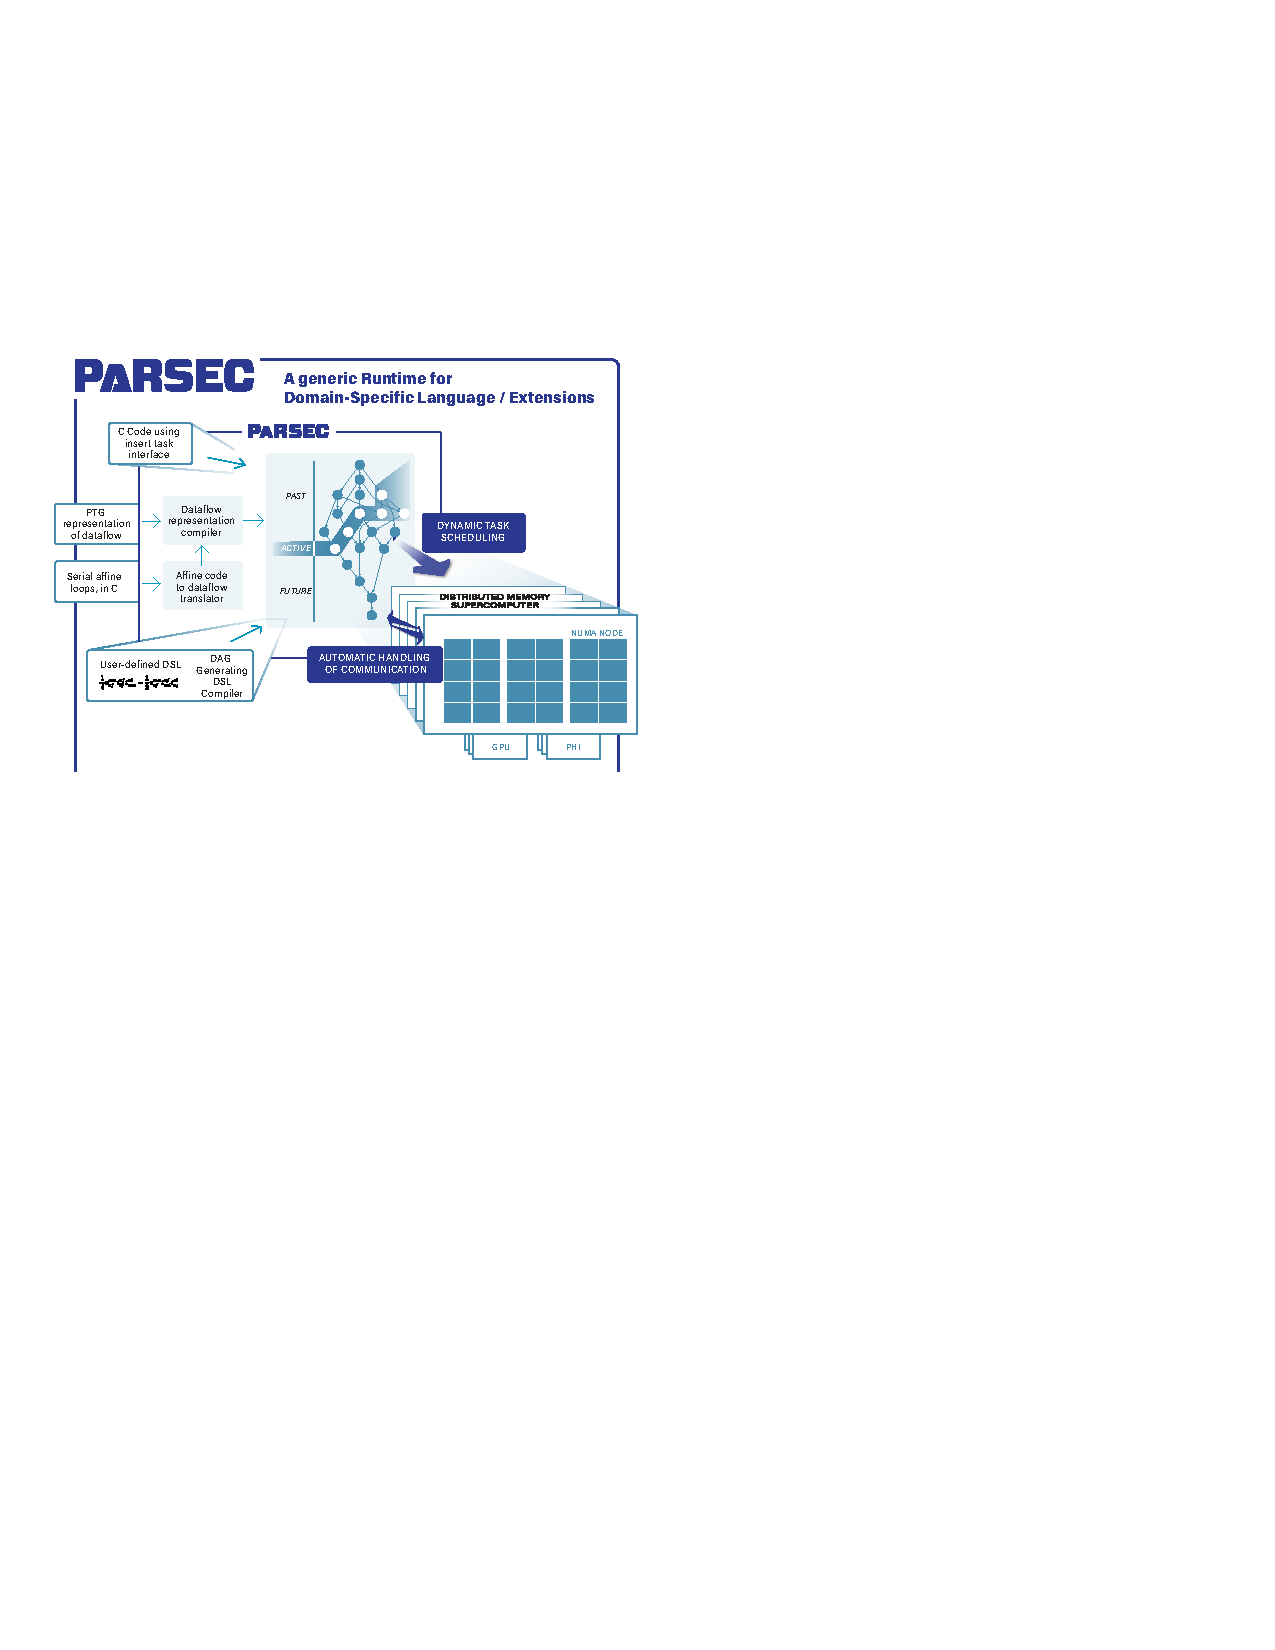
\includegraphics[width=\linewidth]{parsec.pdf}
%%     \end{center}
%%   \end{textblock*}
%% \end{frame}

%% \begin{frame}
%%   \frametitle{Performance Evaluation}

%%   Performance setup:
%%   \begin{itemize}
%%   \item Summit, $\approx$100 GPUs
%%   \item PaRSEC, with local iterators, NVlink support, GPU memory advice
%%   \item libDBCSR, master branch
%%   \end{itemize}

%%   Benchmarks:
%%   \begin{itemize}
%%   \item Synthetic benchmark: random sparsity, random tiling
%%     \begin{itemize}
%%     \item Tiling: average tile size of $1024\times 1024$
%%     \item smallest tile dimension: 512
%%     \item largest tile dimension: 2048
%%     \item[~]
%%     \item Sparsity: fill random (uniform) tiles in the matrix, one by one, until a threshold is reached
%%     \end{itemize}
%%   \item Applicative benchmark: $C_{65}H_{132}$, with 3 possible tilings
%%   \end{itemize}
  
%% \end{frame}

%% \begin{frame}
%%   \frametitle{Synthetic Benchmark}
%%   \relsize{-2}
%%   16 nodes of Summit -- 96 x V100 (GEMM peak: 672 TFlops/s)

%%   PaRSEC: 3 GPU / process, grid of $4\times 8$ processes

%%   libDBCSR: 1 GPU / process, tested all process grids, kept the best for each point
  
%%   \begin{center}
%%     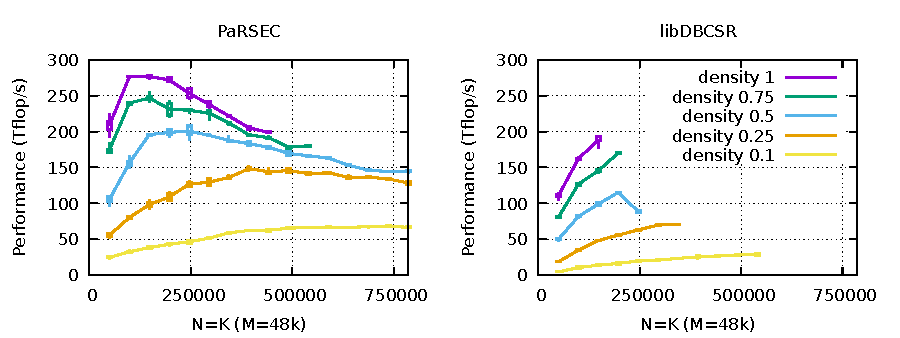
\includegraphics[width=.9\linewidth]{perf-synthetic.pdf}
%%   \end{center}

%%   \flushright\textcolor{orange}{Note: Evaluation stops when libDBCSR could not handle problem size}

%% \end{frame}

%% \begin{frame}
%%   \frametitle{Synthetic Benchmark}
%%   \relsize{-2}
%%   16 nodes of Summit -- 96 x V100 (GEMM peak: 672 TFlops/s)

%%   PaRSEC: 3 GPU / process, grid of $4\times 8$ processes

%%   \begin{columns}
%%     \begin{column}{.45\linewidth}
%%       \begin{center}
%%         Time to completion\\
%%         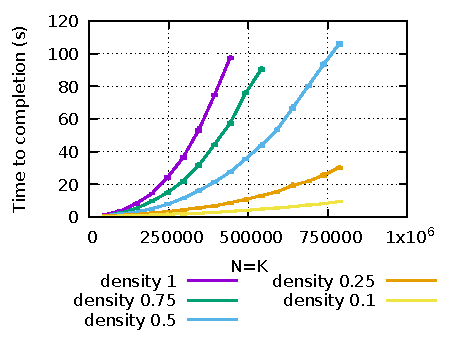
\includegraphics[width=.9\linewidth]{time-synthetic.pdf}
%%       \end{center}
%%     \end{column}
%%     \begin{column}{.45\linewidth}
%%       \begin{center}
%%         Arithmetic Intensity\\
%%         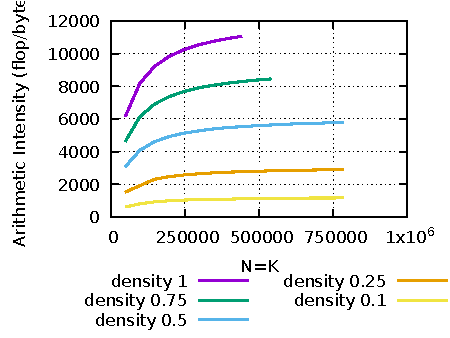
\includegraphics[width=.9\linewidth]{ai-synthetic.pdf}
%%       \end{center}
%%     \end{column}
%%   \end{columns}
%% \end{frame}

\begin{frame}
  \frametitle{$C_{65}H_{132}$}

  \begin{columns}
    \begin{column}{.35\linewidth}
      \begin{center}
        \relsize{-2}
        \begin{tabular}{cc}
          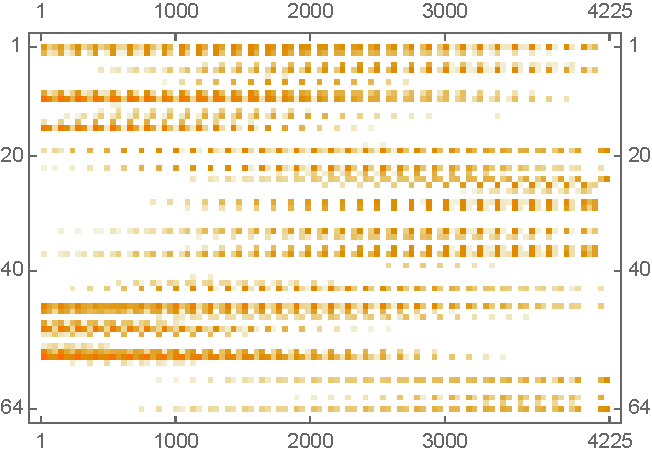
\includegraphics[width=0.45\linewidth]{t2_shape_v1.pdf} & 
          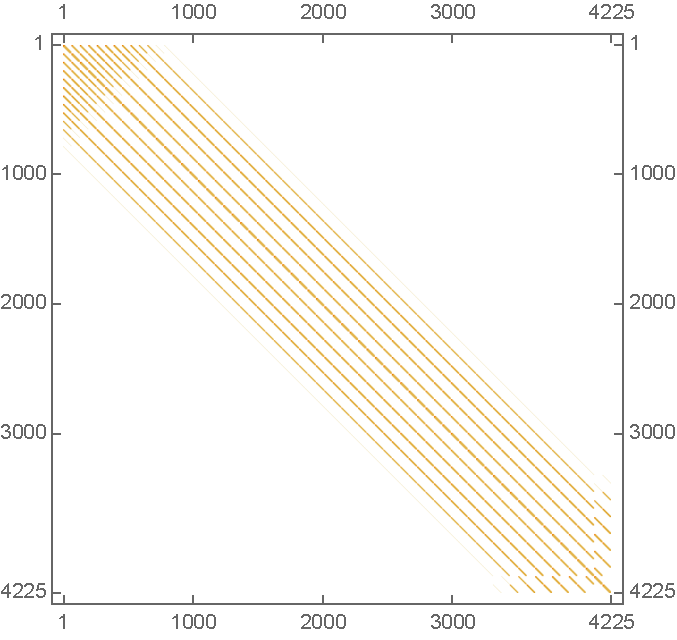
\includegraphics[width=0.45\linewidth]{v_shape_v1.pdf} \\
          $T$ & $V$ \\
          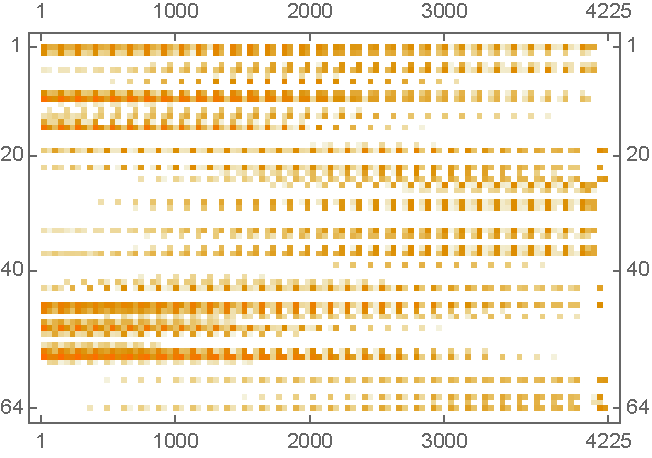
\includegraphics[width=0.45\linewidth]{r_shape_v1.pdf} & 
          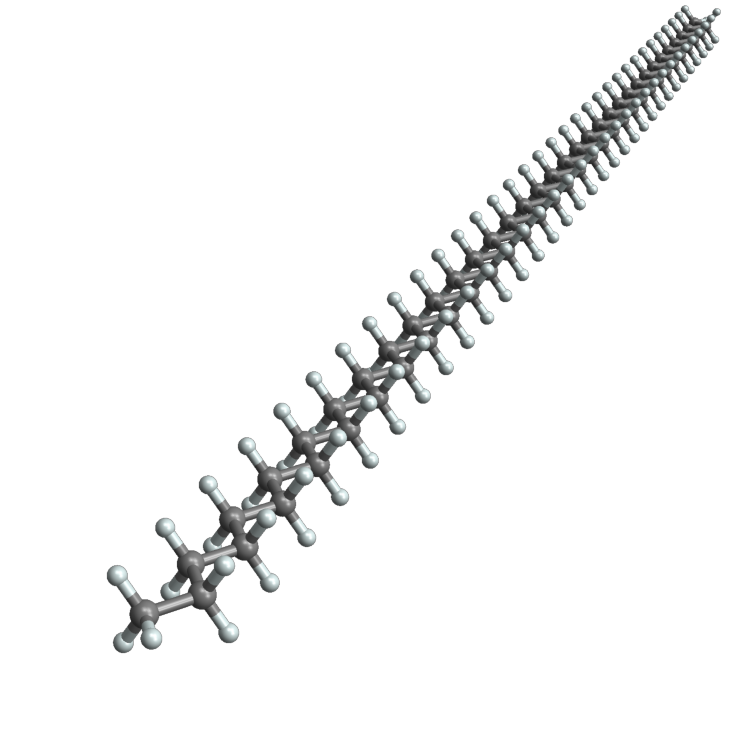
\includegraphics[width=0.45\linewidth]{c65h132.pdf} \\
          $R$ & the \ce{C65H132} molecule \\
        \end{tabular}
        (Tiling v1)
      \end{center}
    \end{column}

    \begin{column}{.5\linewidth}
      \relsize{-2}
      \begin{center}
        \begin{tabular}{l|l|l|l}
          & Tiling $v_1$ & Tiling $v_2$ & Tiling $v_3$ \\\hline
          $M\times N\times K$ & \multicolumn{3}{|c}{$26576\times 2464900 \times 2464900$} \\\hline
          \#flop & 877 Tflop & 923 Tflop & 1237 Tflop \\\hline
          \#flop (opt.) & 850 Tflop & 899 Tflop & 1209 Tflop \\\hline
          \#GEMM tasks & 1899971 & 468368 & 67818 \\\hline
          \#GEMM tasks (opt.) & 1843309 &455159& 66315 \\\hline
          Average \#rows/block & 700 & [500;2500] & [1000;5000]\\\hline
          Average \#col./block & 700 & [500;2500] & [1000;5000]\\\hline
          Density of $T$ & 9.8\% &  10.2\% & 13.2\%\\\hline
          Density of $V$ & 2.4\% & 2.6\% & 3.1\%\\\hline
          Density of $R$ (opt.) & 14.9\% & 16.1\% & 21.7\%\\
        \end{tabular}

        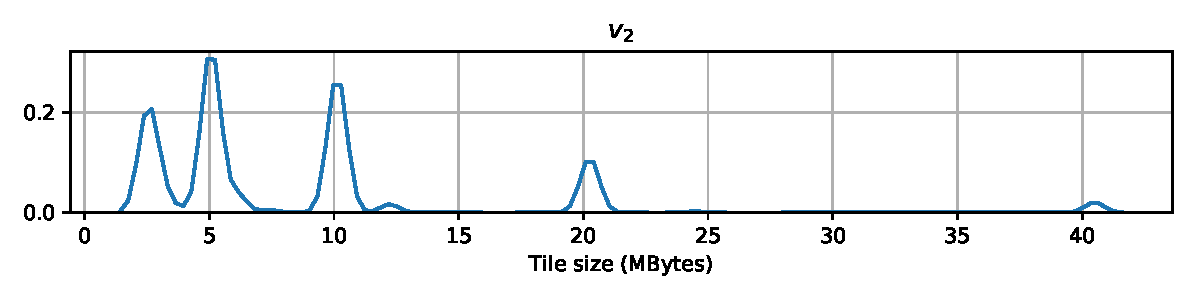
\includegraphics[width=\linewidth]{bs-distrib.pdf}
        
        (Tile size distribution for v2)
      \end{center}
    \end{column}
  \end{columns}
  
\end{frame}

\begin{frame}
  \frametitle{$C_{65}H_{132}$ Strong scaling}

  \begin{columns}
    \begin{column}{.45\linewidth}
      \begin{center}
        Time to completion
        
        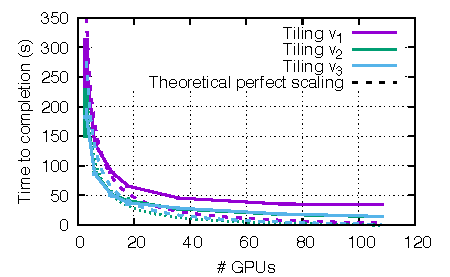
\includegraphics[width=\linewidth]{c65h132-time.pdf}
      \end{center}
    \end{column}
    \begin{column}{.45\linewidth}
      \begin{center}
        Performance
          
          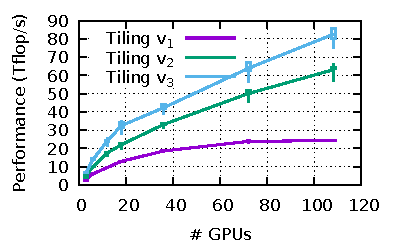
\includegraphics[width=\linewidth]{c65h132-perf.pdf}
      \end{center}
    \end{column}
  \end{columns}
\end{frame}

\begin{frame}
  \frametitle{Conclusion}

  Summary:
  \begin{itemize}
  \item Block-Sparse GEMM product, with irregular tiling, on distributed multi-GPUs, with problems that will not fit the GPU memory
  \item Tensor contraction, application in electronic structure computations
  \item Algorithm: placement of largest data, blocking per memory constraints
  \item Implementation: Problem-specific control flow on top of the basic block-sparse, irregularly tiled GEMM dataflow
  \item Performance: 2x libDBCSR on problems it can handle, can handle much bigger problems
  \item Performance: 35\% parallel efficiency, peak flop is limited by
    sparsity, time to solution less than a minute
  \end{itemize}

  Future work:
  \begin{itemize}
  \item Consider alternative algorithms (generate $B$ tiles multiple times, or cache them)
  \item Model link between tiling and performance, apply selection on which tiles are sent to GPU
  \end{itemize}
  
\end{frame}


